\documentclass[aps,prd,twocolumn,superscriptaddress,nofootinbib,floatfix]{revtex4-2}
\usepackage{amsmath,amssymb,graphicx,hyperref}
\begin{document}
\title{The Shape of the Torus Sets the Sky: SERAPIS Modular Inflation, a String-Loop Tilt and a Parameter-Free Running Test}
\author{Danny Eldridge}
\email{dannyeldridge54@gmail.com}
\affiliation{Independent researcher, Oklahoma City, Oklahoma, USA}
\date{v3.3 draft, 16 November 2026}
\begin{abstract}
We study inflation driven by the shape modulus $\tau$ of a two-torus, with an $SL(2,\mathbb{Z})$-invariant plateau whose vacuum sits at a fixed point of the modular group: the square torus $\tau=i$ or the hexagonal torus $\rho$. A plateau built from $|j-1728|$ leaves the vacuum at $i$ massless; one extra term, of relative strength $\varepsilon\simeq(1.3$--$1.6)\times10^{-4}$, makes it massive and tilts the spectrum. The model then has two faces sharing one closed form, a Janus pair: untilted, $n_s=0.959$--$0.961$ and $r=(3.3$--$3.7)\times10^{-4}$; tilted, $n_s=0.970$--$0.975$, $r=(4.8$--$5.7)\times10^{-4}$ and $\alpha_s\approx-(9$--$10)\times10^{-4}$; with the corrected reheating ($T_R\sim10^6$~GeV) the $\tau=i$ model meets this frozen band only for $\varepsilon\approx(1.40$--$1.45)\times10^{-4}$, at $n_s\approx0.975$. Eliminating the tilt gives a parameter-free relation that predicts $\alpha_s$ from $(n_s,r)$ to about $2\%$, for both vacua (distinguishing it from the attractor value needs $\sigma(\alpha_s)\approx2\times10^{-4}$ and testing the relation itself about $2\times10^{-5}$, both beyond the forecasts for the 2030s), together with $\beta_s=-(3$--$5)\times10^{-5}$, a cap $n_s\le0.985$, $r\le8.3\times10^{-4}$ for any tilt, and a narrow allowed strip in the $(n_s,r)$ plane (for the $j$ and $I_\rho$ plateaus with $N_*=46$--$49$). In a loop-motivated branch, SERAPIS-$E$, the plateau, the vacuum at $\rho$ and the tilt all use the non-holomorphic Eisenstein series $E(\tau,2)$, and the tilt is the one-loop K\"ahler correction of $T^6/(\mathbb{Z}_2\times\mathbb{Z}_2)$ orientifolds with stuck D3 branes, with a natural size; it gives an overlapping $(n_s,r,\alpha_s)$ band, with an $r$ about $4.5$ times below the $p=1$ $j$-based $SL(2,\mathbb{Z})$ attractors of Ref.~\cite{arXiv_2408_05203} at the same K\"ahler metric, as for our own $p=2$ plateau. We follow the history after inflation: reheating through heavy-neutrino decays ($T_R\sim10^6$~GeV at $i$), leptogenesis from inflaton decay at $i$ (a leading-order estimate, conditional on spontaneous CP violation on two cycle classes), and at $\rho$ a residual $\mathbb{Z}_3$ symmetry that makes the inflaton's decay products long-lived, so that the frozen band there requires their decay through string-scale operators; inflaton-based baryogenesis then fails, but Affleck--Dine leptogenesis along $LH_u$, allowed by that $\mathbb{Z}_3$, gives the observed asymmetry inside the frozen band for an essentially massless lightest neutrino, under conditions on the lepton sector (post hoc); the supergravity completion and its TeV-scale wino are discussed in the body. Both vacua and the inflaton path lie on CP-conserving loci, so leptogenesis needs CP violation in the heavy-neutrino couplings; since CP is a symmetry of string effective theories it must be broken spontaneously, and we take it from a racetrack-fixed K\"ahler axion. If generalised CP stays unbroken, inflaton-decay leptogenesis fails and $\delta_{CP}\in\{0,\pi\}$, so a discovery of leptonic CP violation would exclude that version. The tilt at $i$ and $\rho$ is fitted, as is a small symmetry-breaking parameter of the $\rho$ lepton sector, and the plateau itself is placed in the nilpotent sector by choice, as in other $SL(2,\mathbb{Z})$ attractors; we find no string origin for its form. The inflationary predictions were frozen with public hashes and will be scored only on future CMB and large-scale-structure data.
\end{abstract}
\maketitle

\section{Introduction}
Plateau models of inflation, and in particular $\alpha$-attractors~\cite{arXiv_1306_5220}, predict a scalar tilt close to $n_s \simeq 1-2/N_*$ and a small tensor-to-scalar ratio $r$. The latest combined analyses move the preferred tilt upward: CMB data (Planck~\cite{Planck2018X}, ACT DR6~\cite{arXiv_2503_14452}, SPT-3G~\cite{arXiv_2506_20707} with BICEP/Keck~\cite{arXiv_2110_00483}) give $n_s = 0.9682 \pm 0.0032$, and adding DESI DR2 baryon acoustic oscillations~\cite{arXiv_2503_14738} gives $n_s = 0.9728 \pm 0.0029$, with $r < 0.035$ at 95\% confidence~\cite{arXiv_2512_10613}. A plain plateau with $n_s=1-2/N_*$ at $N_* \approx 50$ sits about $4.4\sigma$ below the second value.

Modular-invariant versions of these models, in which the inflaton is the shape modulus $\tau$ of a two-torus and the potential is invariant under $SL(2,\mathbb{Z})$, have been developed in detail~\cite{arXiv_2408_05203,arXiv_2412_19324,arXiv_2405_06497,arXiv_2407_12081,arXiv_2411_18603}. Earlier, Schimmrigk developed automorphic and $j$-inflation, $V\propto|j(\tau)|^2$ on the upper half-plane with a hyperbolic metric of free curvature, with slow roll near $\tau=i$, where $E_6$ vanishes~\cite{arXiv_1512_09082,arXiv_1612_09559}. These models tie inflation to a geometric question: at which shape does the torus come to rest after inflation?

In this paper we study a model, which we call SERAPIS, whose vacuum sits at the square torus $\tau = i$ (and a variant at the hexagonal torus $\rho = e^{2\pi i/3}$). We make five points.
(i) Symmetry alone forces $\tau = i$ to be a critical point and a natural zero of the potential, but a plateau built from $|j-1728|^2$ leaves that vacuum \emph{massless} (Sec.~\ref{sec:setup}).
(ii) A single extra term, $\propto \ln(1+|j-1728|/1728)$, gives the vacuum a mass \emph{and} tilts the plateau. The tilt raises $n_s$ into the range preferred by CMB+DESI while keeping inflation inside a perturbative string-theory bound, $\mathrm{Im}\,\tau \lesssim 25$ (Secs.~\ref{sec:twoterm}--\ref{sec:predictions}).
(iii) With and without this tilt, the model has two ``faces'': an untilted one (Kairos) and a tilted one (Chronos). We derive both in closed form and find a consistency relation that predicts the running $\alpha_s$ from $(n_s, r)$ with no free parameter (Sec.~\ref{sec:janus}).
(iv) We work through a consistency chain covering reheating, supersymmetry breaking, moduli and baryogenesis. Most links pass. Making the supergravity embedding modular-covariant removes the inflaton's F-term and bounds the gravitino mass, pointing to a TeV-scale wino; leptogenesis from inflaton decay works at $\tau=i$, provided the heavy-neutrino couplings carry CP phases, which the CP-conserving vacua cannot supply; at $\rho$ the residual $\mathbb{Z}_3$ closes it (Secs.~\ref{sec:reheating}--\ref{sec:baryo}).
(v) A loop-motivated branch, SERAPIS-$E$, builds plateau, vacuum and tilt from the Eisenstein series $E(\tau,2)$, with the tilt computed from a string one-loop correction (Sec.~\ref{sec:serapisE}).

We are explicit about what is not derived. The size of the tilt parameter, $\varepsilon \simeq (1.3$--$1.6)\times10^{-4}$, was chosen after seeing current data, and we have not found its microscopic origin (Sec.~\ref{sec:limits}). Most ingredients are known: the tilt mechanism is that of singular attractors~\cite{arXiv_2512_02969}, and vacua at $\rho$ appear in Ref.~\cite{arXiv_2408_05203}. What is new is the combination, and the chain of checks around it. The inflationary predictions in Table~\ref{tab:forward} (unmarked rows) are frozen for future data (Sec.~\ref{sec:forward}); numerical computations, except group-theory checks and one disclosed diagnostic (D608), were pre-registered with a hash before they were run.

\section{Modular set-up and what symmetry fixes at $\tau = i$}\label{sec:setup}
We take one complex modulus $\tau = x + i y$ in the upper half plane, with the $\alpha$-attractor K\"ahler potential
\begin{equation}
K = -3\alpha \ln(2\,\mathrm{Im}\,\tau), \qquad \alpha = \tfrac13,
\end{equation}
so the kinetic term is $(\partial x^2 + \partial y^2)/(4y^2)$. Along $x = 0$ the canonical field is $\phi = \ln y/\sqrt{2}$ (reduced Planck units). Following Kallosh and Linde~\cite{arXiv_2408_05203}, the potential is placed in the metric of a nilpotent sector, so any $SL(2,\mathbb{Z})$-invariant function of $\tau$ can serve as $V$.

\paragraph{Stationarity.} The generator $S:\tau\to-1/\tau$ fixes $\tau = i$ and acts there as $\delta\tau \to -\delta\tau$. Hence any $S$-invariant potential that is smooth at $i$ has $\nabla V(i) = 0$. The point $\tau = i$ is therefore always a critical point. This is derived, not chosen. We checked it numerically for every potential used below (D574).

\paragraph{Weight parity.} A modular form of weight $w$ satisfies $f(i) = i^{w} f(i)$, so it vanishes at $i$ unless $w \equiv 0 \pmod 4$. In particular $E_6(i) = 0$ (numerically $|E_6(i)| < 10^{-15}$, with a simple zero), while $E_4(i) = 1.456$. Since $j - 1728 \propto E_6^2/\Delta$, the function $j-1728$ has a \emph{double} zero at $i$ (fitted order $2.000$). In the nilpotent embedding used here $V$ is not derived from a superpotential, so this does not make $\tau=i$ a supersymmetric vacuum of our model; indeed Sec.~\ref{sec:chain} requires $W_0\neq0$ and $F_\tau\neq0$ there. We use only the symmetry statements: $\tau=i$ is a critical point and a double zero of $j-1728$. A de Sitter vacuum cannot sit at $i$ in the minimal heterotic setting~\cite{arXiv_2212_03876}. What symmetry does \emph{not} fix is whether $i$ is a minimum or a saddle, nor the value of the vacuum energy.

\paragraph{The plateau.} We build the plateau from the invariant
\begin{equation}
I(\tau) = \frac{1}{4\pi}\ln\!\left(1 + \frac{|j(\tau)-1728|^2}{1728^2}\right), \qquad V_{\rm pl} = V_0\,\frac{I^p}{I^p+1},
\end{equation}
which vanishes only at $i$ (and its images), is single-valued, and grows as $I \simeq y$ toward the cusp. We use $p = 2$. That is the smallest power for which horizon exit occurs at $y_* \lesssim 25$, inside the bound $\mathrm{Im}\,\tau\lesssim k\,\alpha^{-1}(M_s)\approx29$ that perturbative heterotic thresholds place on a modulus whose threshold grows linearly at the cusp. We impose the stricter cut $y_*\le25$, and we assume the bound applies to $\tau$ when $\tau$ enters the gauge threshold as a $T$-type modulus does (D564, D566).

\paragraph{A flaw: the vacuum is massless.} Because $|j - 1728|^2 \propto |\tau - i|^4$, the plateau rises as $V_{\rm pl} \propto |\tau - i|^{4p}$ near the vacuum: quartic for $p=1$ and octic for $p=2$ (fitted exponents $4.00$ and $8.00$). The vacuum has no quadratic term, so no mass. After inflation the field oscillates anharmonically, with equation of state $w = (n-2)/(n+2) = 3/5$~\cite{Turner1983} for $n = 8$, and this changes the inflationary e-fold count $N_*$. Earlier predictions that assumed matter-like reheating must be revised (D567a). Section~\ref{sec:twoterm} supplies the missing mass.

\section{The two-term model: one term for the vacuum mass and the tilt}\label{sec:twoterm}
A quadratic vacuum needs a term $\propto |\tau - i|^2$. Taking the \emph{first} power of $|j-1728|$ instead of the square gives one:
\begin{gather}
I_1(\tau) = \frac{1}{4\pi}\ln\!\left(1 + \frac{|j(\tau)-1728|}{1728}\right), \nonumber\\
V = V_0\left[\frac{I^2}{I^2+1} + \varepsilon\, I_1\right].
\label{eq:twoterm}
\end{gather}
Near $i$ the new term is quadratic and isotropic (fitted exponent $2.00$ in both directions), so it gives the vacuum a mass. Toward the cusp it grows as $I_1 \simeq y/2$, which tilts the plateau upward (D575).

Using $I_1$ alone with $p=1$ would also give a massive vacuum, but inflation would then start at $y_* \approx 213$--$227$, far outside the string bound. In the family $V = f(I^p)$ a massive vacuum needs $p\cdot(\text{power of }|j-1728|) = 1$, while staying inside the bound needs $p \geq 2$. No member has both. The two-term form~(\ref{eq:twoterm}) breaks this trade-off (D574, D575).

\paragraph{Exponential tilt, not a log tilt.} In terms of $\phi$, the term $\varepsilon I_1 \simeq (\varepsilon/2)\,e^{\sqrt2\phi}$ is an \emph{exponential} ramp. It carries both slope and positive curvature, $V_{\phi\phi} \simeq \varepsilon y$. A logarithmic ``lift'' of the plateau, $I^{2\delta}$, adds only slope. Matching slopes at horizon exit gives $\varepsilon \simeq 4\delta/y_*$. The curvature is what makes the allowed window narrow, and it produces the running signature of Sec.~\ref{sec:janus} (D576). The tilt mechanism itself is that of singular attractors~\cite{arXiv_2512_02969}. What is specific here is that the \emph{same} term supplies the vacuum mass at $\tau = i$.

\paragraph{Mass without tilt.} For comparison, a one-loop species-scale term, $\kappa\,y^2|\hat G_2|^2/N^2$ with $N = -6\ln(2y|\eta|^4)+\tilde N_0$~\cite{arXiv_2407_12081,arXiv_2507_05345}, is also quadratic at $i$ (since $\hat G_2(i) = 0$). It leaves $n_s$ unchanged to $<4\times10^{-4}$ for $\kappa \le 10^{-2}$ (D577). The untilted face of the model with this mass is the ``Kairos'' branch. The two-term model is the tilted ``Chronos'' branch.

\paragraph{The window for $\varepsilon$.} We require all of the following at once:
\begin{itemize}
\item horizon exit inside the string bound, $y_* \le 25$;
\item $n_s$ within $2\sigma$ of CMB+DESI;
\item the reheating history of Sec.~\ref{sec:reheating}, evaluated with exact numerics.
\end{itemize}
These fix $\varepsilon \in [1.3, 1.6]\times10^{-4}$ (D602). The window is only about 25--30\% wide, and $\varepsilon$ is a post-hoc parameter. We return to its origin in Sec.~\ref{sec:limits}.

\section{Predictions from exact numerics}\label{sec:predictions}
We solve the background exactly and integrate the Mukhanov--Sasaki equations for scalar and tensor modes, with Bunch--Davies initial conditions at $k/aH = 200$, evaluated at $k/aH = 10^{-3}$. $N_*$ is counted exactly back from $\epsilon_H = 1$ (D588).

\paragraph{Slow-roll accuracy.} At fixed $y_*$ the slow-roll e-fold count is about $1.7$ e-folds short. In $n_s$, this error largely cancels against the first-order slow-roll error in the $n_s$ formula. The net exact-minus-slow-roll shift is only $\Delta n_s = -0.0002$ to $-0.0004$, with $r$ higher by 2--3\% and $y_*$ lower by about $0.4$ (D587, D588). The code reproduces the attractor limit to within $0.002$ in $n_s$.

\paragraph{Results.} With the reheating bracket of Sec.~\ref{sec:reheating} as first estimated ($N_* \approx 46$--$49$; the corrected reheating of Sec.~\ref{sec:reheating} keeps only $\varepsilon\approx(1.40$--$1.45)\times10^{-4}$ in the frozen band, D815):
\begin{itemize}
\item \textbf{Chronos} (two-term, $\varepsilon = 1.3$--$1.6\times10^{-4}$): $n_s = 0.970$--$0.975$ and $r = 4.8$--$5.7\times10^{-4}$, with horizon exit at $y_* = 23$--$24.5$, and $\alpha_s=-(8.8$--$10.2)\times10^{-4}$ (D642).
\item \textbf{Kairos} (untilted): $n_s = 0.959$--$0.961$ and $r = 3.3$--$3.7\times10^{-4}$, with $y_* = 21.9$--$22.6$ (D637). These use the Chronos reheating bracket. With a mass from the species-scale term alone, the octic phase ends at a point set by the free coefficient $\kappa$; a later switch raises $N_*$ by $-\tfrac18\ln(\rho_x'/\rho_x)$, where $\rho_x$ and $\rho_x'$ are the energy densities at which the octic phase ends without and with the later switch, i.e.\ by up to a few e-folds for a very light mass, and moves Kairos's $n_s$ up by about $0.0008$ per e-fold (D644).
\end{itemize}
Against current data (Fig.~\ref{fig:nsr}), Chronos lies within about $1\sigma$ of CMB+DESI and within $2.3\sigma$ of CMB alone. Kairos lies $2.2$--$3.0\sigma$ below the CMB value and $4.0$--$4.9\sigma$ below CMB+DESI (D602, D637). Whether the upward shift of $n_s$ with BAO data is physical or reflects the mild tension between DESI BAO and the CMB in $\Lambda$CDM is debated~\cite{arXiv_2503_14738}; since $\varepsilon$ was chosen with this shift in view, Chronos stands or falls with it.

\begin{figure}[tbp]
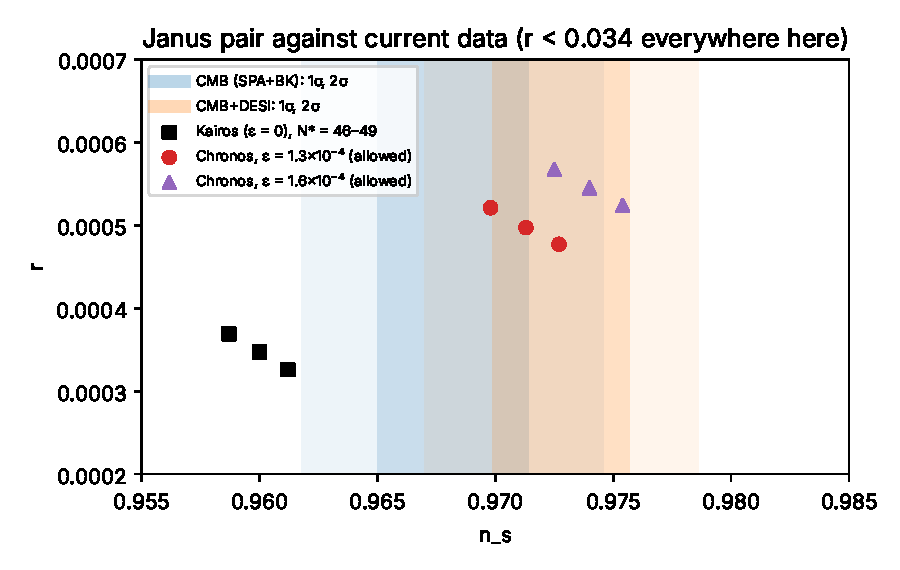
\includegraphics[width=\columnwidth]{figs/fig2_ns_r.pdf}
\caption{Kairos (squares) and Chronos (circles, triangles) against the CMB and CMB+DESI $n_s$ bands~\cite{arXiv_2512_10613}. Each Chronos point is one reheating bracket ($T_R = 10^3$ or $10^5$~GeV, stiff or matter bound); all satisfy $y_* \le 25$.}
\label{fig:nsr}
\end{figure}

\begin{figure}[tbp]
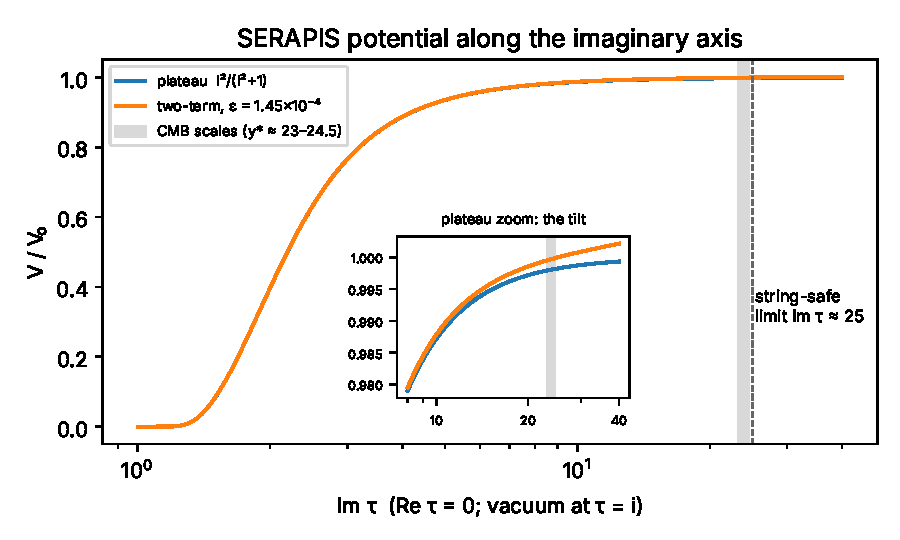
\includegraphics[width=\columnwidth]{figs/fig1_potential.pdf}
\caption{The two-term potential along $\mathrm{Im}\,\tau$. Inset: the tilt on the plateau. Shaded: horizon exit of CMB scales. Dashed: the perturbative bound $\mathrm{Im}\,\tau \approx 25$.}
\label{fig:pot}
\end{figure}

\section{The Janus pair in closed form}\label{sec:janus}
Near the cusp, $I \simeq y$ and $I_1 \simeq y/2$, so Eq.~(\ref{eq:twoterm}) reduces to $V/V_0 \simeq 1 - y^{-2} + (\varepsilon/2)y$. With $\phi = \ln y/\sqrt2$,
\begin{equation}
N = \int \frac{y\,dy}{4 + \varepsilon y^3}.
\end{equation}
Define the tilt fraction $x \equiv \varepsilon y_*^3/4$. To leading order,
\begin{align}
1 - n_s &= \frac{16}{y_*^2}\left(1 - \frac{x}{2}\right), &
r &= \frac{64}{y_*^4}(1+x)^2, \nonumber\\
\alpha_s &= -\frac{128}{y_*^4}\left(1+\frac{x}{4}\right)(1+x).
\end{align}
Kairos is $x = 0$, with $y_*^2 = 8N_*$: $1-n_s = 2/N_*$, $r = 1/N_*^2$ and $\alpha_s = -2/N_*^2$. Since $V\propto I^2/(I^2+1)$ with $I\simeq y$ behaves as $1-y^{-2}=1-e^{-2\sqrt2\phi}$, the effective attractor parameter is $\alpha_{\rm eff}=1/12$ (so $r=12\alpha_{\rm eff}/N_*^2$), not the $\alpha=1/3$ of the K\"ahler potential. Chronos, in its allowed window, has $x \approx 0.31$--$0.47$. These leading-order forms neglect the constant offsets of $I$ and $I_1$ (see the last paragraph of this section): for Kairos the exact $r$ is 22--26\% below $1/N_*^2$ (D637), while $n_s$ is accurate to about $0.002$. A single parameter carries the model from one face to the other: the tilt raises $n_s$, raises $r$, and makes the running more negative.

\paragraph{Running signature.} Compared with an attractor with the \emph{same} $n_s$, the running is enhanced by
\begin{equation}
\mathcal{R}(x) = \frac{(1+x/4)(1+x)}{(1-x/2)^2},
\end{equation}
which equals $1$ for Kairos and about $2.8$ at $x = 0.47$. The exact numerics give $\alpha_s = -(8.8$--$10.2)\times10^{-4}$ for Chronos at $N_*=46$--$49$. That is $2.2$--$3.0$ times the attractor value $-(1-n_s)^2/2$ (Fig.~\ref{fig:run}; D632, D642). The $\rho$ variant gives the same signature (ratio $2.1$--$2.3$; D634).

\paragraph{Consistency relation.} With three observables and two parameters, one combination is fixed:
\begin{gather}
\varrho = \frac{2\sqrt r}{1-n_s},\quad x = \frac{\varrho-1}{1+\varrho/2},\quad A = \frac{1-n_s}{1-x/2}, \nonumber\\
\alpha_s = -\frac{A^2}{2}\left(1+\frac{x}{4}\right)(1+x).
\label{eq:consistency}
\end{gather}
Measured $(n_s, r)$ thus predict $\alpha_s$ with no free parameter, for either vacuum. Against the exact Mukhanov--Sasaki results, Eq.~(\ref{eq:consistency}) is accurate to $11$--$13\%$ in every case, a uniform bias (D635).

\paragraph{Removing the bias.} The bias comes from the constant offsets of the invariants. Since $|j-1728|\simeq e^{2\pi y}$, one has $I\simeq y-c$ with $c=\ln1728/2\pi=1.1865$, and $I_1\simeq I/2$ exactly, so the offset enters only through the field map $\phi=\ln(I+c)/\sqrt2$. To first order in $u\equiv1/I_*$, with $x=\varepsilon I_*^3/4$,
\begin{gather}
1-n_s = 8u^2\left[(2-x)+cu(5-x)\right], \nonumber\\ r = 64u^4(1+x)^2(1+2cu), \nonumber\\
\alpha_s = -32u^4(1+x)\left[(4+x)+cu(23+2x)\right].
\label{eq:consistency2}
\end{gather}
Solving the first two for $(u,x)$ from measured $(n_s,r)$ and evaluating the third reproduces the exact $\alpha_s$ to $0.2$--$0.4\%$ at all eight test points, for both faces; $c$ is fixed by $j$, so the relation remains parameter-free. Part of this agreement is a cancellation between neglected orders: the full first-order slow-roll map of the asymptotic potential, inverted the same way, gives $1.1$--$1.6\%$ and recovers the input $\varepsilon$ to within $1\%$ (D640). We quote $\sim2\%$ as the accuracy. The same closed form, applied to the exact $\rho$-variant spectra, predicts their running to $1.0\%$, and the full map to $1.4\%$, recovering $\varepsilon=6.0\times10^{-5}$; one relation serves both vacua (D666).

\paragraph{The Janus curve.} The predictions themselves also follow in closed form from $(N_*,\varepsilon)$. With the end of inflation at $I_e\simeq\sqrt2$,
\begin{equation}
N_*=\int_{\sqrt2}^{I_*}\frac{I^3\,dI}{(I+c)^2(4+\varepsilon I^3)}\;\xrightarrow{c\to0}\;\frac{I_*^2}{8}\,{}_2F_1\!\left(1,\tfrac23;\tfrac53;-x\right),
\end{equation}
which fixes $(I_*,x)$ and, through Eq.~(\ref{eq:consistency2}), $n_s$, $r$ and $\alpha_s$. Against the exact spectra this reproduces $n_s$ to $+0.0005$--$0.0008$ (the known slow-roll e-fold offset), $r$ to $2$--$4\%$ and $\alpha_s$ to $3\%$; dropping the offset $c$ degrades $n_s$ by $\sim0.005$ (D673). Along the curve at $N_*=47.6$, $n_s$ rises from $0.9605$ ($x=0$) through $0.9745$ ($x=0.5$) to $1$ at $x\simeq2.1$, where the ramp balances the plateau. Requiring horizon exit inside the string bound, $y_*\le25$, caps the tilt for \emph{any} $\varepsilon$. At $N_*=47.6$ the closed form gives $x\le0.67$ and $n_s\lesssim0.978$, conservative by about $0.003$ because it overestimates $y_*$ by $\simeq0.4$. The exact spectra at the bound give $n_s\le0.9836$ and $r\le8.2\times10^{-4}$ at $N_*=46$, and $n_s\le0.9795$ and $r\le6.1\times10^{-4}$ at $N_*=49$ (D674); a smaller $N_*$ permits a larger $\varepsilon$ at the bound. The $\rho$ variant gives the same cap, $n_s\le0.9844$ and $r\le8.3\times10^{-4}$ (D676). A measurement of $n_s>0.985$ would therefore exclude the whole SERAPIS family with $y_*\le25$ and $N_*=46$--$49$ (the post-hoc self-diluted $\rho$ history of Sec.~\ref{sec:limits}, superseded as $\rho$'s preferred route by D895, lies outside these bounds), at both vacua and independently of the tilt strength. We froze this cap (locks D675, D677). More sharply, the family fills a narrow strip in the $(n_s,r)$ plane (Fig.~\ref{fig:strip}): computing the exact spectra along both edges of the reheating bracket from $\varepsilon=0$ to the cap, the allowed $r$ at fixed $n_s$ spans at most $21\%$, e.g.\ $r=(4.4$--$5.3)\times10^{-4}$ at $n_s=0.970$ (D678). The $\rho$ variant fills the same strip to within $2.2\%$ (D680), so the strip is a property of the modular plateau rather than of the vacuum. Its height comes only from the reheating bracket, so within the family a joint $(n_s,r)$ measurement reads off $N_*$: $dr/dN_*\approx3\times10^{-5}$ per e-fold, and $N_*$ shifts by $0.76$ per decade of $T_R$, so $\sigma(r)\approx2\times10^{-5}$ would fix the reheating temperature to about a decade for a given post-inflationary equation of state (D682). This lies beyond planned experiments. A joint $(n_s,r)$ measurement off the strip excludes the family even when each value alone lies in its range (locks D679, D681).

\begin{figure}[tbp]
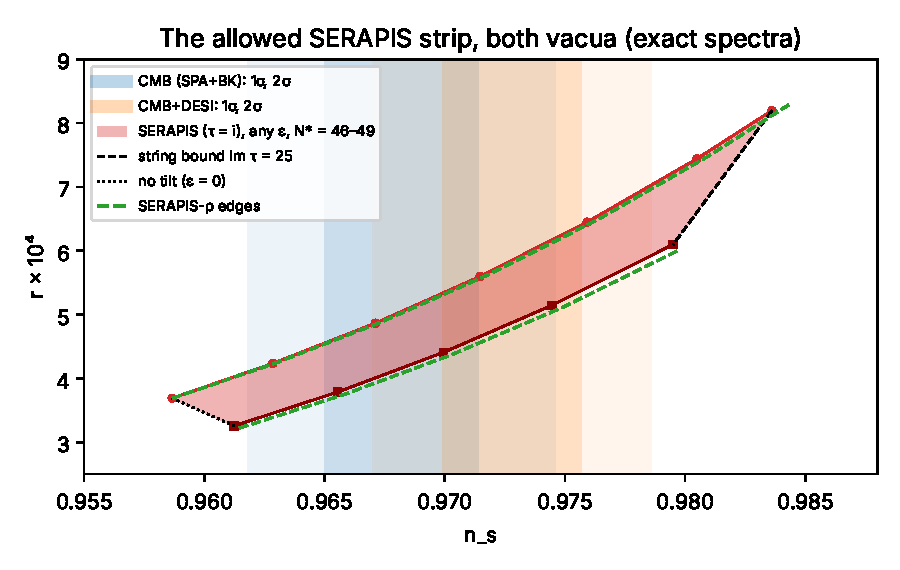
\includegraphics[width=\columnwidth]{figs/fig5_strip.pdf}
\caption{The allowed strip of SERAPIS for any $\varepsilon$: $\tau=i$ (shaded) from exact spectra along the edges $N_*=46$ (circles) and $N_*=49$ (squares), closed by the untilted points (dotted) and the string bound (dashed); the green dashed lines are the exact edges of the $\rho$ variant. Shown against the CMB and CMB+DESI $n_s$ bands~\cite{arXiv_2512_10613}.}
\label{fig:strip}
\end{figure}

\paragraph{A general relation.} Nothing above is specific to the modular invariants. For any potential $V\simeq1-Ae^{-p\phi}+\delta e^{q\phi}$, with $\kappa=q/p$ and $x$ the ratio of ramp to plateau slope at horizon exit, the same steps give $1-n_s=2pA'(1-\kappa x)$, $r=8A'^2(1+x)^2$, $\alpha_s=-2p^2A'^2(1+x)(1+\kappa^2x)$, hence
\begin{gather}
\varrho=\frac{p\sqrt{r/2}}{1-n_s},\qquad x=\frac{\varrho-1}{1+\kappa\varrho}, \nonumber\\
\alpha_s=-\frac{(1-n_s)^2}{2}\,\frac{(1+x)(1+\kappa^2x)}{(1-\kappa x)^2}.
\end{gather}
SERAPIS is $(p,\kappa)=(2\sqrt2,\tfrac12)$. For the power-law singular T-models of Ref.~\cite{arXiv_2512_02969} ($p=\sqrt{2/3\alpha}$, $\kappa=\beta$) the relation reproduces exact slow-roll running to better than $1\%$ (D669). Measuring $(n_s,r,\alpha_s)$ therefore tests the whole class of plateaus with an exponential ramp and, through $\kappa$, distinguishes its members. In the modular construction $\kappa$ is not free: every logarithm of a modular form grows linearly in $y$, so $q=\sqrt2$, while a plateau $I^n/(I^n+1)$ gives $p=n\sqrt2$, hence $\kappa=1/n$ whichever invariant supplies the tilt. Treating $n$ as unknown, the exact spectra of both vacua return $n=2.18$--$2.20$ for the true $n=2$, the offset being the leading-order bias (D672); the three observables would thus measure the plateau power itself.

\paragraph{Running of the running.} The same map fixes the next coefficient. To leading order,
\begin{equation}
\beta_s\equiv\frac{d^2n_s}{d\ln k^2}=128\,u^6(1+x)\left(2x^2-5x-16\right),
\label{eq:beta}
\end{equation}
which reduces to the attractor value $-4/N_*^3$ at $x=0$. For the general family it reads $\beta_s=-\tfrac14(1-n_s)^3(1+x)\left[(1-\kappa x)(1+\kappa^2x)+(1+x)(1-\kappa^3x)\right]/(1-\kappa x)^3$, which reproduces exact slow-roll values for the singular T-models to better than $1\%$ (D671). The exact spectra give $\beta_s=-(3.0$--$4.6)\times10^{-5}$ for both vacua at $N_*=46$--$49$, and the full slow-roll map predicts them to within $17\%$ (D666). This band, and the relation between all four observables, were frozen before any measurement could test them (lock D667).

\begin{figure}[tbp]
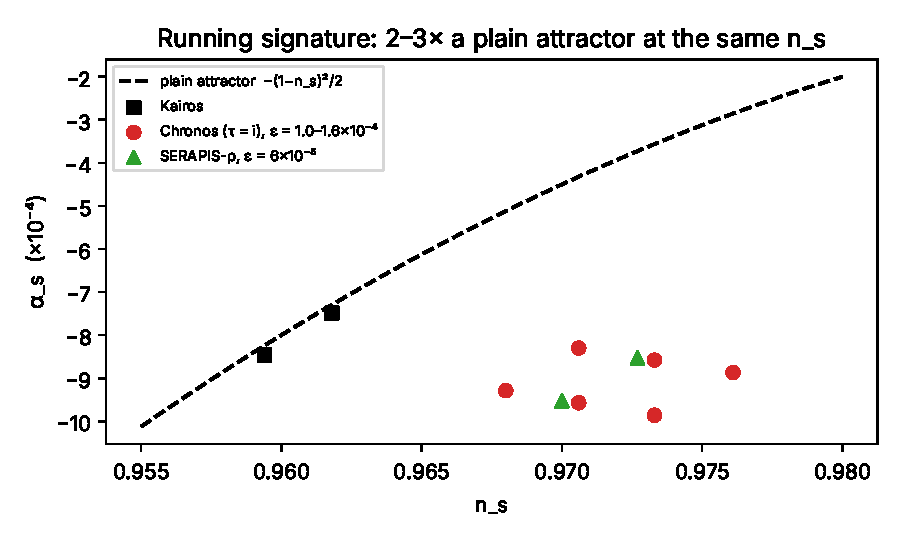
\includegraphics[width=\columnwidth]{figs/fig3_running.pdf}
\caption{Running versus $n_s$. Dashed: the plain attractor relation. SERAPIS with the exponential tilt lies a factor $2$--$3$ below it at fixed $n_s$.}
\label{fig:run}
\end{figure}

\section{After inflation: a stiff phase and a nearly sterile inflaton}\label{sec:reheating}
\paragraph{Stiff phase.} Near $\tau = i$ the plateau term rises as $\delta^8$ (Sec.~\ref{sec:setup}), and the $\varepsilon I_1$ term adds a small quadratic piece. The inflaton therefore first oscillates in the octic part, with $w = 3/5$. It reaches the quadratic regime only after the energy density has fallen by a factor $\rho_x/\rho_{\rm end} \approx 2\times10^{-6}$ (D578). The exact background confirms this: the effective $w$ is $0.556$ over the first e-fold after inflation and $0.537$ over the next 1.5 e-folds (Fig.~\ref{fig:w}; D595).

\paragraph{A nearly sterile inflaton.} Every physical mass is a modular invariant, so by the stationarity argument of Sec.~\ref{sec:setup} it is stationary at $\tau = i$. After canonical normalisation, the linear couplings of the inflaton to the following all vanish there (D589a, D601):
\begin{itemize}
\item the mass of any particle--antiparticle pair;
\item kinetic couplings, which reduce to currents whose on-shell matrix element is $\propto(m_1^2 - m_2^2) = 0$;
\item the trace of the stress tensor;
\item the conformal anomaly.
\end{itemize}
Linear decays survive only through off-diagonal couplings between states of the same flavour multiplet with \emph{different} masses, and these scale with the mass splitting. The heaviest split multiplet dominates the decay. For heavy neutrinos with generic splittings this gives $T_R \sim 10^3$--$10^5$~GeV. That is above the sphaleron scale but far below the usual gravitational-decay estimate. \emph{Correction (D727):} this scaling holds for states whose mass eigenvalues have the same sign. The $\Gamma_2$ doublet's mass matrix is traceless, with eigenvalues $\pm s$, so the rotation of its eigenvectors couples the pair with strength $2s\,\theta'$, an axion-like (pseudoscalar) coupling that is not suppressed by any splitting ($\kappa=1.26$, confirmed by two independent numerical methods). With this channel $T_R\approx(0.8$--$3)\times10^6$~GeV, which raises $N_*$ by an estimated $1$--$3$ e-folds relative to the bracket below. The frozen predictions were computed with the earlier bracket and are kept as frozen; recomputed with exact spectra at $T_R=10^6$--$3\times10^6$~GeV (D729, D815), $\varepsilon=1.3\times10^{-4}$ gives $n_s=0.9719$--$0.9736$, $r=(4.7$--$4.9)\times10^{-4}$ and $\varepsilon=1.6\times10^{-4}$ gives $n_s=0.9746$--$0.9764$, $r=(5.2$--$5.4)\times10^{-4}$, all with $y_*\le24.8$; the stiff-phase rows leave the frozen band (low $r$ at the smaller $\varepsilon$, $n_s>0.975$ at the larger), while the matter-like rows stay inside. The decay is $10^{15}$--$10^{16}$ times slower than the expansion rate when the octic phase ends, so the stiff-phase rows describe the actual history (D730). The corrected $\tau=i$ prediction therefore meets the frozen band only for $\varepsilon\approx(1.40$--$1.45)\times10^{-4}$ (exact spectra on a $0.05\times10^{-4}$ grid, D815), at $n_s\approx0.9745$--$0.9750$, $r\approx(4.85$--$4.93)\times10^{-4}$. Two faster channels must be closed, because instant reheating would raise $N_*$ by about $6$--$9$ e-folds and move Chronos to $n_s\approx0.976$--$0.98$ and $y_*>25$, outside both the frozen band and the string bound. (i) \emph{Preheating.} Quadratic couplings $g^2\phi^2\chi^2$ are not forbidden by stationarity; for a field whose invariant mass is $m_0^2(1+a|\delta|^2)$, $g^2=a\,m_0^2/M_P^2$. For $a=1$ the resonance parameter is $q\lesssim2\times10^{-4}$ for every field with $m_0\lesssim m_\phi$, while the fields with $q\sim1$ have $m_0\sim10^{13}$~GeV$\gg\omega$ and evolve adiabatically. Broad resonance therefore does not occur, and non-resonant transfer is below $10^{-13}$ of the inflaton energy for $m_0\le10^{11}$~GeV. Self-resonance of the inflaton is slow for a plateau of Planckian width~\cite{arXiv_1710_06851} and can only move $w$ toward $1/3$, inside the bracket used for $N_*$. (ii) \emph{Gravitino plus inflatino.} With the goldstino projected out, the inflatino mass at $\tau=i$ is $\tfrac43m_{3/2}$, so in the constant-$W_0$ embedding $\phi\to\psi_{3/2}\tilde\chi$ is open only for $m_{3/2}<m_\phi/(1+\tfrac43)\approx9\times10^{10}$~GeV, excluded by the gravitino condition of Sec.~\ref{sec:chain} (a naive projection with a thin margin). In the covariant completion the inflaton carries no F-term and this channel is not sourced at leading order. Both statements are estimates (D641); the frozen predictions assume them.

\paragraph{The e-fold count.} We bracket the history in two ways. The stiff phase is taken either at its octic value ($w = 3/5$) or conservatively as matter-like ($w = 0$), followed by a matter phase down to $T_R$. Using the standard matching~\cite{arXiv_astro-ph_0305263} this gives $N_* = 46$--$49$ (D602), which is the range used in Sec.~\ref{sec:predictions}; at $\tau=i$ it is superseded by the corrected reheating below (D727, D815).

\begin{figure}[tbp]
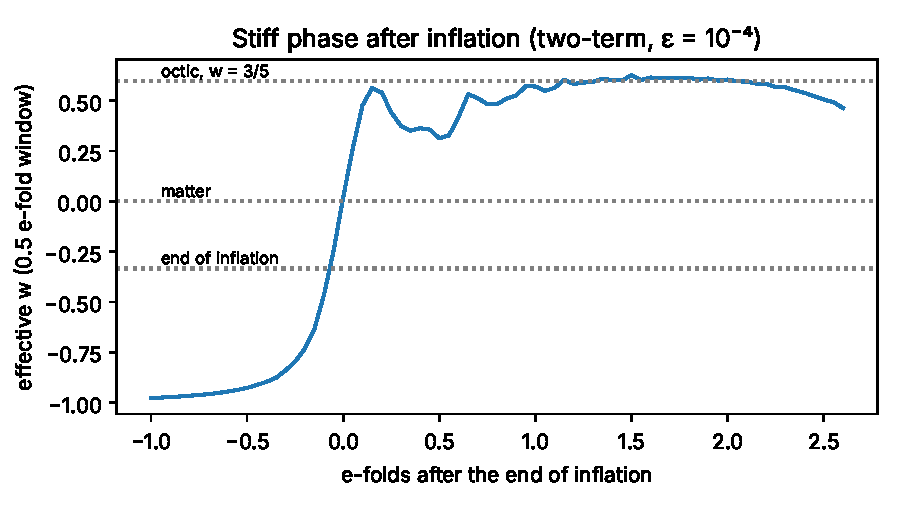
\includegraphics[width=\columnwidth]{figs/fig4_w.pdf}
\caption{Effective equation of state (fit over a $0.5$ e-fold window) through the end of inflation. It settles near the octic value $w = 3/5$ before the quadratic term takes over.}
\label{fig:w}
\end{figure}

\section{Consistency chain}\label{sec:chain}
We list the checks a complete model must pass, with their status. Numbers refer to the $\tau = i$ model; the $\rho$ variant is in Sec.~\ref{sec:rho}.

\paragraph{Supersymmetry breaking: the covariant completion.} Kallosh and Linde embed the plateau with a nilpotent field $X$ and a constant superpotential $W_0$~\cite{arXiv_2408_05203}. A constant $W_0$ has no modular weight, so $G=K+\ln|W|^2$ is not $SL(2,\mathbb Z)$ invariant, and the inflaton then acquires an F-term, $F_\tau\propto K_\tau W_0\neq0$ at $\tau=i$. The minimal invariant completion for $K=-\ln(2\,\mathrm{Im}\,\tau)$ is $W=(W_0+fX)\,\eta(\tau)^{-2}$, of weight $-1$, for which $G=-\ln(2y|\eta|^4)+\ln|W_0+fX|^2$. Its $\tau$-dependence is the invariant $L(\tau)$, which is stationary at both fixed points; numerically $G_\tau=3\times10^{-25}$ at $i$ and $-8\times10^{-26}$ at $\rho$ (D647). In this completion, which we adopt because it respects the symmetry used throughout the paper:
\begin{itemize}
\item the inflaton carries \emph{no} supersymmetry breaking ($F_\tau=0$; all of it sits in $X$, with $f^2=3|W_0|^2$ for $\Lambda=0$), so the inflaton-to-gravitino problem of moduli decays does not arise at leading order and no lower bound on $m_{3/2}$ follows from it;
\item the F-term potential $V_F=m_{3/2}^2M_P^2\,e^{L-L(i)}\,4y^2|\partial_\tau L|^2$ vanishes at $i$ but grows as $e^{\pi y/3}$ toward the cusp. Keeping the plateau intact by absorbing it into the metric of $X$ requires the $X$ F-term to stay positive, which gives $m_{3/2}\lesssim2.6\times10^6$~GeV if the field starts at $y\simeq26$, 6--12 e-folds before horizon exit, and $m_{3/2}\lesssim(0.6$--$1.3)\times10^7$~GeV if it starts at $y_*$ (D649, D658). This construction puts the plateau in by hand, as in Ref.~\cite{arXiv_2408_05203}; beyond $y\simeq26$ the potential simply steepens; without that freedom, $|\Delta n_s|<10^{-3}$ requires $m_{3/2}\lesssim3$--$8$~TeV (D648);
\item visible scalars receive $m_Q^2=m_{3/2}^2$ for every modular weight (D647), and tree-level $A$-terms vanish at $\tau=i$ (see Sec.~\ref{sec:baryo}). If the gauge kinetic functions do not depend on $X$, gaugino masses are anomaly-mediated, $|M_{1,2,3}|\simeq(8.8,2.7,19)\times10^{-3}\,m_{3/2}$, with a wino LSP (D650).
\end{itemize}
These requirements define a window. The gluino bound $\gtrsim2.3$~TeV and the disappearing-track bound on a wino LSP, $670$~GeV~\cite{arXiv_2603_08315} (superseding $660$~GeV~\cite{arXiv_2201_02472}), require $m_{3/2}\gtrsim2.5\times10^5$~GeV. A thermal wino relic not exceeding the dark-matter density ($M_2\lesssim2.9$~TeV; freeze-out lies well below $T_R$) requires $m_{3/2}\lesssim1.1\times10^6$~GeV. Both lie inside the positivity bound. If the higgsino mass is of order $m_{3/2}$, its threshold contribution to $M_2$ is comparable to the anomaly-mediated one, so these window ends are uncertain by a factor of about two. The covariant completion therefore predicts a wino LSP at $0.67$--$1.85$~TeV for an Einasto halo, a sub-component of the dark matter, since gamma-ray line searches exclude $1.85$~TeV up to the thermal mass~\cite{arXiv_2507_15934}; correspondingly scalars at $m_{3/2}\simeq(2.5$--$7)\times10^5$~GeV and a gluino at $4.7$--$13$~TeV (for cored halos the wino may reach $2.9$~TeV, with $m_{3/2}$ up to $1.1\times10^6$~GeV and the gluino up to $21$~TeV). A $125$~GeV Higgs boson with negligible stop mixing at $M_S\sim10^5$--$10^6$~GeV then needs a moderate $\tan\beta$~\cite{arXiv_1407_4081}. Because $G_\tau=0$ and every other linear coupling of the inflaton vanishes at the fixed point, the decay $\phi\to2\psi_{3/2}$ is absent at linear order. Thermally produced gravitinos ($Y_{3/2}\lesssim2\times10^{-17}$ at these $T_R$) decay within $2\times10^{-3}$~s, before nucleosynthesis, and their winos are negligible (D651). These are estimates.

\paragraph{The constant-$W_0$ embedding.} For comparison, with a constant $W_0$ the inflaton carries one third of $|F|^2$ and no residual symmetry forbids its decay to gravitinos, which with the standard rate~\cite{arXiv_hep-ph_0611166} overproduces them unless $m_{3/2}>m_\phi/2\approx10^{11}$~GeV (D584). A single modulus is not of no-scale type ($K^{\tau\bar\tau}K_\tau K_{\bar\tau}=1$ rather than $3$~\cite{arXiv_1305_1247}), and tree-level soft masses are $m_Q^2=(1-k)\,m_{3/2}^2$ for matter of modular weight $k$ (D639, D643). They vanish only for $k=1$, which with the weight-parity rule of Sec.~\ref{sec:setup} requires flavour multiplets with suitable representations for the Yukawa couplings not to vanish at $i$. Loop-induced masses are then $3\times10^8$--$10^{10}$~GeV, just below the Higgs-mass bound $M_S\lesssim2\times10^{10}$~GeV~\cite{arXiv_1407_4081}. This was the chain frozen in the $\tau=i$ lock (D605); it relies on a superpotential that breaks the modular symmetry.

\paragraph{Other moduli.} The inflation scale exceeds the gravitino mass ($H_{\rm inf}/m_{3/2}\approx37$ for constant $W_0$, $\gtrsim10^6$ in the covariant completion). Stabilising the dilaton the way KKLT does would therefore fail~\cite{arXiv_hep-th_0411011}. A supersymmetric racetrack with $W_Y = W_Y' = 0$ avoids this, with a parameter window spanning a factor of about 100 (D586, D591). A heavy dilaton decays to superpartners, and the lightest superpartner (LSP), stable under the matter parity below, could overclose the universe. Adiabatic tracking suppresses the dilaton's leftover oscillation energy as $f_Y \propto (m_Y/H)^{-8}$ to $(m_Y/H)^{-20}$. We compute the stiff-phase growth directly ($\times 8.6$) and fix the Hubble-induced coefficient by supergravity ($c = \sqrt2$). The LSP bound is then met for $m_Y \gtrsim 140\,H_{\rm end}$, about $7\times10^{14}$~GeV (D592--D596). This bound was derived for the constant-$W_0$ spectrum. In the covariant completion the LSP is a TeV wino that freezes out at $T_f\approx M_2/20\lesssim150$~GeV, below $T_R$, so winos made directly in dilaton decays re-thermalise. Gravitinos from $Y\to2\psi_{3/2}$, however, decay after freeze-out, which relaxes the bound to $m_Y\gtrsim35\,H_{\rm end}\approx2\times10^{14}$~GeV at the vacuum, inside the racetrack window (D652, D658).

\paragraph{Proton stability.} In the constant-$W_0$ embedding a matter parity carried by the centre of the modular group, a $\mathbb{Z}_4^R$ or $\mathbb{Z}_8^R$ symmetry, forbids dimension-4 baryon-number violation (D528--D533). It passes the anomaly check, and it is compatible with the selection rule at $\tau = i$ (D551). In the covariant completion this mechanism is lost. Since $\eta^{-2}$ is invariant under the centre $-I$, the superpotential is centre-neutral and the centre symmetry is no longer an $R$-symmetry. With the $\eta^{-2}$ multiplier, couplings are non-zero at $i$ only if their matter weights sum to $0\bmod4$ ($0\bmod6$ at $\rho$). No anomaly-free assignment survives that also forbids dimension-5 operators (D656, D657). This is specific to the symmetries the modular centre can supply ($\mathbb{Z}_4$, $\mathbb{Z}_8$): an anomaly-free non-$R$ symmetry that forbids the dangerous operators while allowing the Yukawa couplings exists, proton hexality, but it is a $\mathbb{Z}_6$, and non-$R$ symmetries cannot also solve the $\mu$ problem~\cite{arXiv_1102_3595} (D657a). The centre can still supply \emph{ordinary} matter parity, which forbids dimension-4 operators only. At $\rho$ every anomaly-free assignment of this kind keeps all required couplings non-zero (D661). At $\tau=i$ none does (D661, D662), for a simple reason: matter parity needs odd weights for quarks and leptons and even weights for the Higgs fields, so the Weinberg operator has $2k_L+2k_{H_u}\equiv2\bmod4$ and vanishes at $i$, as does a singlet Majorana mass (D663). At $\tau=i$ the covariant completion therefore needs flavour multiplets with non-trivial $\rho(S)$. This assumes singlet couplings of trivial character built from level-one forms; couplings with other characters (e.g.\ $\eta^4$, of weight two and non-zero at $i$) are not excluded. The $\Gamma_2\simeq S_3$ structure of Sec.~\ref{sec:baryo} provides them: $-I\in\Gamma(2)$ acts trivially on its representations, so the centre parity is unchanged, while with lepton and heavy-neutrino doublets the weight-two doublet form, non-zero at $i$, gives a Weinberg operator of full rank (leptons as $\mathbf2\oplus\mathbf1$) and a non-vanishing Majorana mass, both exactly degenerate within the doublet at $\tau=i$ (D664). This degeneracy matters for reheating: the off-diagonal decays that set $T_R$ (Sec.~\ref{sec:reheating}) need a mass splitting, which must then come from a $\mathbf2\oplus\mathbf1$ heavy-neutrino structure or another split multiplet. A $\mathbf2\oplus\mathbf1$ heavy-neutrino structure, the same one the lepton sector already needs, supplies it: the doublet--singlet coupling through the weight-two form splits the pair by $\Delta M/M\approx0.08$--$0.5$ for an order-one coupling, which with the unsuppressed decay of Sec.~\ref{sec:reheating} gives $T_R\approx(0.8$--$3)\times10^6$~GeV independently of the splitting (D727, superseding the $T_R\sim10^5$~GeV estimate of D690). At $\rho$ no doublets are needed. Planck-suppressed dimension-5 operators $c\,QQQL/M_P$, dressed by the wino with scalars at $10^5$--$10^6$~GeV, need $c\lesssim5\times10^{-3}$--$2\times10^{-2}$ (an estimate; natural if the coefficients carry Yukawa suppression). In that embedding, dimension-5 operators reappear only with $M_{\rm eff} \sim M_P^2/m_{3/2}\approx6\times10^{25}$~GeV, safely above the bound (D542, D585).

\paragraph{The axion partner.} $\mathrm{Re}\,\tau$ is massless during inflation, which Ref.~\cite{arXiv_2503_14904} warns can produce isocurvature. Here the inflationary path is CP-symmetric, so the axion enters the curvature perturbation only at second order. A two-field $\delta N$ computation gives an isocurvature contribution $\sim 10^{-8}$ of $\zeta$ (D582, D587). At the vacuum the Hessian is isotropic, so the axion decays together with the inflaton.

\section{Baryogenesis and a neutrino-mass prediction}\label{sec:baryo}
\paragraph{Leptogenesis from inflaton decay at $\tau=i$.} Section~\ref{sec:reheating} shows that diagonal decays to heavy-neutrino pairs vanish at $\tau = i$. Off-diagonal decays to $N_1N_2$ exist. In a minimal $\Gamma_2 \simeq S_3$ flavour model the coupling is $\kappa = 1.26$ (D597). But the coupling scales with the mass splitting, while the resonant CP asymmetry needs a small splitting. The asymmetry therefore saturates at $Y_B \approx 1.25\times10^{-11}$, a factor of 7 short of the observed $8.75\times10^{-11}$. Higher-weight doublets reduce the shortfall to a factor of $1.75$ but do not close it (D598). \emph{Correction (D728):} that conclusion relied on the coupling scaling with the splitting, which does not hold for this doublet (Sec.~\ref{sec:reheating}, D727). With the unsuppressed decay, $T_R\approx(0.8$--$3)\times10^6$~GeV does not depend on the splitting, and the same estimate gives $Y_B\ge8.75\times10^{-11}$ for all $\Delta M/M$ from $10^{-8}$ up to $0.014$--$0.5$, the upper limit rising with $M/m_\phi$ from $0.1$ to $0.45$. However, the consistent $\mathbf2\oplus\mathbf1$ structure at $\tau=i$ splits the light pair by $\Delta M/M\approx0.6$--$11$, not the $0.08$--$0.5$ estimated earlier, and then only one corner passes ($Y_B\approx9.7\times10^{-11}$ at $M/m_\phi=0.33$); with the doublet alone $\Delta M=0$ and $\varepsilon=0$ (D738). This assumes a maximal CP phase and neglects washout ($T_R/M\sim5\times10^{-5}$). With an exactly degenerate doublet the asymmetry is restored by radiative splitting: running from a high scale splits the pair and the $\tau$ Yukawa supplies the phase~\cite{BrancoRadLepto2005}; with a third heavy neutrino and $\tan\beta\ge5$, $Y_B\ge8.75\times10^{-11}$ for 34--86\% of a Casas--Ibarra grid at $T_R\approx3\times10^6$~GeV (leading-order estimate, D744--D745), so inflaton-decay leptogenesis is viable at $\tau=i$ without the tuned light-neutrino mass that Affleck--Dine requires. Related modular constructions use other fixed points or vacua~\cite{arXiv_2411_18603,arXiv_2604_04585}.

\paragraph{Where the CP phase comes from.} Both vacua and the SERAPIS-$E$ path $\mathrm{Re}\,\tau=\tfrac12$ lie on the CP-conserving locus of generalised CP combined with modular symmetry (the imaginary axis and the boundary of the fundamental domain)~\cite{arXiv_1905_11970}. If generalised CP is imposed, every coupling is real there, the leptogenesis asymmetry vanishes on both branches, and $\delta_{CP}\in\{0,\pi\}$ (D762); at $\rho$ the post-hoc $LH_u$ Affleck--Dine route of Sec.~\ref{sec:limits} needs instead a spontaneous phase of the condensate (the superseded self-diluted history needed none). The passes above therefore assume CP phases in the heavy-neutrino couplings. These are high-energy phases: in the radiative estimate the low-energy mixing matrix drops out of $H=Y^\dagger Y$, the pass fraction is $68$--$71\%$ for any $\delta_{CP}$, and with real couplings nothing passes (D763). A flux-stabilised second modulus might seem a natural source, since a flux relation $U_2U_3=c$ fixes $U_3$ off its CP locus for most rational $c$ when $U_2=\omega$~\cite{arXiv_2405_18813} (D764, D766). In untwisted $T^6/(\mathbb{Z}_2\times\mathbb{Z}_2)$ flux vacua, however, every supersymmetric Minkowski point of this kind also involves the third torus (the model of Ref.~\cite{arXiv_2405_18813} fixes it to the dilaton), because a superpotential independent of the inflaton torus admits only a real dilaton at such a point (D772, D773). A relation involving the inflaton doubles its K\"ahler metric and raises $r$ to $(6.5$--$7.5)\times10^{-4}$, outside the frozen band (D765). In a string completion, however, CP is a symmetry of the effective theory (an outer automorphism of the modular group~\cite{arXiv_2010_10782,arXiv_1901_03251}), so the phases cannot be free couplings: CP must be broken spontaneously, and in our toroidal configuration no flux-fixed modulus does so (D843, D844). We therefore take the phase from a K\"ahler-modulus axion fixed by a racetrack with real coefficients, $W=W_0+Ae^{2\pi iT/N_1}+Be^{2\pi iT/N_2}$, which has CP-odd minima in $90\%$ of the cases we scanned (one modulus, before uplift); in about $40\%$ of them a CP-odd minimum is the deepest, otherwise it lies within about $5\%$ of the deepest (D845, D851). This is a postulate of the model (D846). If the heavy-neutrino masses are generated by D-instantons on that cycle, a common phase can be rotated away, so they must come from at least two instanton sectors of different charge; the physical phase $2\pi\Delta n\,\langle\mathrm{Re}\,T\rangle$ then has $|\sin|>0.1$ in $80\%$ of the CP-odd vacua (D852). At $\tau=i$ the resonant pair is a flavour doublet whose members share one brane charge and hence one instanton phase; on a single cycle class, mixing with the singlet adds no relative phase, so this branch needs CP-odd axions on two cycle classes (D854). The $\rho$ branch does not use this phase: its frozen band has no baryogenesis mechanism, and its post-hoc history needs none (D792, D855). The leptogenesis phase follows from that vacuum rather than from a uniform prior. The model therefore predicts no particular $\delta_{CP}$, but a discovery of leptonic CP violation by DUNE or Hyper-Kamiokande would exclude its generalised-CP version. At $i$ no Affleck--Dine twin exists, unlike SERAPIS-$E$ at $\rho$: the potential is isotropic about $i$ to leading order ($|j-1728|\simeq c|z|^2(1+O(|z|^2))$; D795), so an off-axis orbit carries a charge, but the residual symmetry is only $\mathbb{Z}_2$ and the Majorana parity eigenstates it decays into cannot store it (D794).

\paragraph{Affleck--Dine along $LH_u$.} Our low reheating temperature is the regime where Affleck--Dine leptogenesis~\cite{AffleckDine1985,arXiv_hep-ph_9507453} along the $LH_u$ flat direction~\cite{arXiv_hep-ph_9310297} is usually effective, with an asymmetry set mainly by the lightest neutrino mass~\cite{arXiv_hep-ph_0102187,arXiv_hep-ph_0109154}. Two features of $\tau=i$ make it work here. First, the tree-level $A$-terms vanish: $A=F^\tau\partial_\tau\ln\hat y$, where the physical coupling $\hat y$ is modular invariant up to a constant phase, so by the stationarity argument of Sec.~\ref{sec:setup} $\partial_\tau\hat y(i)=0$ whenever $\hat y(i)\neq0$ (checked numerically, D646). The $A$-term is therefore of loop size, as in the standard analyses, even in the constant-$W_0$ embedding where $m_{3/2}\gg m_{\rm soft}$. Second, with $m_{\rm soft}\sim m_{3/2}\lesssim10^6$~GeV (covariant completion) or loop-size soft masses (constant $W_0$, if below $H_x$), the flat direction starts to oscillate at $H\sim m_{\rm soft}$, after the stiff phase has ended ($H_x\approx5\times10^9$~GeV), in a matter-dominated background (D600).

We integrated the flat direction numerically in a matter-dominated background, with $W=(LH_u)^2/2M$, $M=v_u^2/m_{\nu_1}$, Hubble-induced mass and $A$-terms of order one ($c_H=|a_H|=1$, assumed, from a Kähler coupling to $X$) and an $A$-term of order $m_{\rm soft}$. The asymmetry parameter $Q=\mathrm{Im}(\psi^*\dot\psi)/h^2$ is $0.014$--$0.087$ over the relative phase, and the yield is independent of $m_{\rm soft}$. Including the factor two from $L=H_u=\phi/\sqrt2$, the observed $n_B/s$ requires $m_{\nu_1}\simeq1.6\times10^{-10}$--$2.7\times10^{-9}$~eV at the corrected reheating temperature $T_R=(0.8$--$3)\times10^6$~GeV (D900; $2\times10^{-13}$--$9\times10^{-11}$~eV at the earlier $T_R=10^3$--$10^5$~GeV, D646, D646a). Thermal effects are negligible here: at the onset the plasma temperature is $\sim10^9$~GeV while $\phi_{\rm osc}/T\gtrsim5\times10^4$, so the fields coupled to $\phi$ are heavy and the two-loop thermal logarithm is below $2\times10^{-4}$ of the soft term (D653, D900). The large $M\gg M_P$ requires a symmetry that forbids $(LH_u)^2/M_P$. With the $\eta^{-2}$ multiplier a singlet Weinberg operator is non-zero at $\tau=i$ when $k_L+k_{H_u}\equiv0\bmod2$, e.g.\ $k_L=k_{H_u}=1$ with coefficient $E_4\,\eta^{-2}$ (D654a). That operator is allowed, so nothing in the modular structure suppresses it: at Planck size it would give $m\sim2\times10^{-5}$~eV along every direction. Affleck--Dine at $i$ therefore needs, as at $\rho$, an instanton-only Weinberg term (action $S\gtrsim13$--$17$ for $\Lambda=M_s$), and in addition a lightest seesaw mass $\lesssim3\times10^{-9}$~eV, which the minimal $2\oplus1$ texture does not give ($m_1\approx5\times10^{-5}$--$4\times10^{-3}$~eV, D786). At $i$ it is thus a conditional alternative to the inflaton-decay leptogenesis above (D903).

\paragraph{Consequence.} If Affleck--Dine is the source, baryogenesis requires an essentially massless lightest neutrino, $m_{\nu_1}\approx2\times10^{-10}$--$3\times10^{-9}$~eV at $\tau=i$ and $2\times10^{-11}$--$9\times10^{-10}$~eV at $\rho$ (D895, D900); with the inflaton-decay routes above this is no longer required. The mass ordering is not predicted. With normal ordering, which current oscillation data mildly favour~\cite{arXiv_2410_05380}, this gives $\sum m_\nu\simeq0.0587$~eV, at the 95\% upper limit $\sum m_\nu < 0.0592$~eV from DESI DR2 with the Lyman-$\alpha$ forest in $\Lambda$CDM (Ref.~\cite{arXiv_2607_27410}, Sec.~VI.D.2), alive by $0.0005$~eV; a combination adding DES Year-5 supernovae gives $<0.052$~eV with a prior extending to zero, below the floor, but $<0.092$~eV with a hierarchy-informed prior~\cite{arXiv_2606_17994}. This floor is shared by every normal-ordering $\Lambda$CDM model, so it tests that class rather than SERAPIS specifically, and current data prefer an effective $\sum m_\nu<0$~\cite{arXiv_2610_20977}; with inverted ordering it would give $\simeq0.10$~eV. If $m_{\nu_1}$ is left free at $\tau=i$, the range is $0.059$--$0.064$~eV (D786). A measurement of $\sum m_\nu \gtrsim 0.07$~eV would remove this route to baryogenesis (D604).

\section{The hexagonal variant: SERAPIS-$\rho$}\label{sec:rho}
The same structure can be built with the vacuum at $\rho = e^{2\pi i/3}$ from ingredients with a more direct string pedigree. The plateau uses $I_\rho = (1/4\pi)\ln(1+|j|^2/1728^2)$, which vanishes at $\rho$~\cite{arXiv_2408_05203}; the same invariant $|j|^2$ is the potential of $j$-inflation~\cite{arXiv_1612_09559}. The mass and tilt come from the threshold/species function $L = -\ln(2y|\eta|^4)$~\cite{arXiv_2407_12081,arXiv_2411_08467}:
\begin{equation}
V = V_0\left[\frac{I_\rho^2}{I_\rho^2+1} + \varepsilon\,(L - L(\rho))\right].
\end{equation}
$L$ has an isotropic minimum at $\rho$ (Hessian $0.667$ in both directions), while at $i$ it has a saddle (D608). Inflation runs along $\mathrm{Re}\,\tau = 1/2$. Because $L$ rises toward the cusp about twice as steeply as $I_1$, the allowed value is $\varepsilon = 6\times10^{-5}$. Like $\varepsilon$ in the $\tau = i$ model, this value was chosen after seeing the data (D610).

With its own reheating history (a plateau term $\propto\delta^{12}$, hence $w = 5/7$) the predictions are $n_s = 0.969$--$0.972$, $r = 4.6$--$5.1\times10^{-4}$ and $\alpha_s = -(8.5$--$9.5)\times10^{-4}$ (D613, D634). These frozen values come from first-order slow roll; exact spectra at the same $N_*$ give $n_s=0.9691$--$0.9722$, $r=(4.67$--$5.16)\times10^{-4}$ and $\alpha_s=-(8.7$--$9.9)\times10^{-4}$, the same band to rounding except that the largest $r$ lies $1.2\%$ and the most negative $\alpha_s$ about $4\%$ beyond the frozen edges (D816). These are essentially indistinguishable from the $\tau = i$ model. In the constant-$W_0$ embedding the proton parity survives at $\rho$ under its selection rule (D612). In the covariant completion the centre still supplies ordinary matter parity at $\rho$ with all required couplings non-zero (D661), which is an advantage of the $\rho$ variant over $\tau=i$. The residual $\mathbb{Z}_3$ at $\rho$ (Sec.~\ref{sec:limits}) applies to this vacuum as well: the inflaton is $\mathbb{Z}_3$-charged, so the same long-lived decay products and the same lack of baryogenesis in the frozen band follow. Otherwise the chain carries over with $m_\phi \approx 7\times10^{10}$~GeV, $m_{3/2} \gtrsim 3.6\times10^{10}$~GeV and soft masses of about $2\times10^8$~GeV (D614; constant-$W_0$ embedding). We found the combination nowhere in the literature we checked; each ingredient is prior art (D611). As discussed in Sec.~\ref{sec:limits}, the linear-in-$L$ term is not itself derived. On present evidence the $\rho$ variant is nonetheless the better-motivated vacuum. Its tilt function is the universal heterotic $N=2$ threshold, and in the covariant completion the modular centre gives it ordinary matter parity without extra flavour structure. Its observables coincide with those of the $\tau=i$ model (D688). The covariant completion works identically at $\rho$ ($G_\tau(\rho)=0$), with the same gravitino bound, $m_{3/2}\lesssim2.6\times10^6$~GeV at $y\simeq26$ (D655), so the superpartner window of Sec.~\ref{sec:chain} carries over.

\section{A loop-motivated branch: SERAPIS-$E$}\label{sec:serapisE}
Lattice sums single out $\rho$ (equivalently its image $e^{i\pi/3}$ on the line $\mathrm{Re}\,\tau=\tfrac12$). For any sum $\sum' f(|m+n\tau|^2/\mathrm{Im}\,\tau)$ with $f$ completely monotone (a positive mixture of Gaussians), which includes $E(\tau,s)$ and, in the Kronecker limit, $-\ln(2\,\mathrm{Im}\,\tau|\eta|^4)$, the hexagonal lattice is the unique minimiser at fixed covolume~\cite{Rankin1953,Montgomery1988,arXiv_1504_01153}; at $i$ both $E(\tau,2)$ and that threshold are saddles, descending along the arc toward $\rho$ (D801). In the orientifold used below this requires equal numbers of stuck branes at the three half-periods, which $SL(2,\mathbb{Z})/\Gamma(2)\simeq S_3$ permutes: each half-period sum carries a sign character and is invariant only under an index-three subgroup, and only the symmetric total collapses to $-\tfrac34E(U,2)$. A Scherk--Schwarz breaking reduces the group in the same way; in a heterotic free-fermionic example the one-loop energy, a difference of shifted lattice sums, is invariant under a subgroup of $\Gamma^0(2)$ type ($b$ even, containing the stabiliser $TST^{-1}$ of $1+i$; the source labels it $\Gamma_1(2)$), which has no order-three fixed point, and has a metastable AdS minimum at $1+i$, an image of $i$~\cite{arXiv_2504_19364}. We cite it only as an existence proof of a reduced-group minimum at an image of $i$. With the full $SL(2,\mathbb{Z})$, a vacuum at $i$ needs a hand-built function such as $|j-1728|$, which is why we regard the $\rho$ branch as the better-motivated one there (D801, D803).

The open problem of $\varepsilon$ (Sec.~\ref{sec:limits}) can be addressed with a computed string correction. In $T^6/(\mathbb{Z}_2\times\mathbb{Z}_2)$ orientifolds the one-loop Kähler potential of Berg, Haack and Körs~\cite{BHK2005} depends on the torus shape through the non-holomorphic Eisenstein series $E(U,2)=\sum'(\mathrm{Im}\,U)^2/|m+nU|^4$. With D3 branes at the half-periods the sum over positions collapses to $-\tfrac34E(U,2)$, giving $K^{(1)}=(15N/64\pi^6)\,E(U,2)/(\mathrm{Im}\,S\,\mathrm{Im}\,\rho)$ (D689). The function $E(\tau,2)$ is modular invariant, has its global minimum at $\rho$, and grows as $2\zeta(4)y^2$ toward the cusp. We therefore consider
\begin{equation}
\frac{V}{V_0}=\frac{\hat E}{\hat E+1}\,\bigl(1+C\hat E\bigr),\quad \hat E=E(\tau,2)-E(\rho,2),
\end{equation}
with $C=15N/(64\pi^6\,\mathrm{Im}\,S\,\mathrm{Im}\,\rho)$,
in which the plateau, the vacuum at $\rho$ and the tilt all use the same one-loop object.

\paragraph{Reheating at $\rho$.} The vacuum is heavy, $m_\phi\approx2.2\times10^{13}$~GeV ($m^2/H^2\approx35$), so the inflaton oscillates quadratically from the start and we froze the predictions below with $N_*=48.4$--$49.9$, from an estimate of sterile-decay reheating, $T_R\sim10^6$--$10^8$~GeV (D692). Later checks revise this. At $\rho$ the weight-two $\Gamma_2$ heavy-neutrino doublet has one massless state, and the inflaton couples linearly to it, so it is not sterile there. With the doublet alone, $\phi\to N_2N_2$ reheats to $T_R\approx7\times10^8$--$7\times10^{10}$~GeV ($N_*\approx50.0$--$51.5$, $n_s=0.9731$--$0.9746$ from exact spectra, D817), but $N_2$ cannot thermalise and the universe becomes dominated by dark radiation, which rules that minimal sector out. A $\mathbf2\oplus\mathbf1$ sector whose singlet mixes through the weight-two doublet gives every state a mass at $\rho$ and removes the problem, at the cost of a reheating history that depends on that sector (D720--D724). In that sector the degenerate light pair splits linearly away from $\rho$, which reheats the universe to $T_R\approx3\times10^8$--$3\times10^9$~GeV with $n_s=0.9729$--$0.9736$ and $r=(4.66$--$4.75)\times10^{-4}$ (exact spectra), inside the frozen band (D725, D814). Leptogenesis from these decays (D775--D776) is superseded: the residual $\mathbb{Z}_3$ makes the decay products long-lived and dilutes any early asymmetry (Sec.~\ref{sec:limits}).

\paragraph{Predictions.} Exact Mukhanov--Sasaki spectra give, for $C=(1.0$--$1.3)\times10^{-6}$, i.e.\ $\mathrm{Im}\,S\,\mathrm{Im}\,\rho\approx750$--$975$ for the flux-free tadpole-consistent placement (absent the uplift anti-D3; see below) of five stuck D3 branes at each half-period and one at the origin, the tilt measuring the excess $N-N_0=4$ (D696)\footnote{$\mathrm{Im}\,S\,\mathrm{Im}\,\rho\approx375$--$488$ if a stuck brane counts as half a unit, or with exotic O3 planes. In the $\mathcal N=1$ orientifold the $E_2(0,U)$ term is also generated, suppressed by the other two K\"ahler moduli instead of $S$~\cite{BHK2005}, so $C$ collects both channels. The one-loop K\"ahler potential of this IIB orientifold contains only $E_2$-type functions, so this tilt, unlike those of the $\tau=i$ and $\rho$ variants, has a loop origin here (D756).},
\begin{align}
n_s&=0.970\text{--}0.975,\qquad r=(4.6\text{--}5.1)\times10^{-4},\nonumber\\
\alpha_s&=-(9.4\text{--}10.6)\times10^{-4}.
\end{align}
At $n_s=0.970$ the model gives $r=4.75\times10^{-4}$, inside the frozen strip of Fig.~\ref{fig:strip}; without the tilt ($C=0$) it reproduces the untilted attractor, $n_s\approx0.961$, $r\approx3.6\times10^{-4}$. Because both the plateau correction and the tilt scale as $e^{\mp2\sqrt2\phi}$, it is the $\kappa=1$ member of the Janus family; the general relation with $p=2\sqrt2$ predicts its running to 3.5--5\% (D692). Observationally SERAPIS-$E$ is therefore the same family as SERAPIS. What it adds is a microscopic origin for the tilt, with a natural, not tuned, size. Three caveats remain: the Eisenstein plateau is placed in the uplift sector by hand, although only its approach $1-a/\hat E$ matters: a different interior form shifts $n_s$ by $<0.001$ and $r$ by $<2\%$, and $a$ is absorbed into $C$ (D698); the formula is specific to this orientifold; and the one-loop potential itself pushes the D3 stacks from the half-periods toward the origin, where the tilt changes sign, with a Hubble-scale tachyonic mass, $m_A^2\approx-(0.1$--$1)H^2$ (estimate, D694). The stacks must therefore be held at the half-periods by a stronger effect, such as stuck D3 branes at the fixed points, which have no position moduli and carry no twisted RR charge~\cite{MaidenShiuStefanski2006} (D695; the D3 tadpole $3N+N_0+N_{\rm flux}=16$ is satisfied by this placement and the K-theory probe conditions are trivially met by D3 branes, D696; with the uplift's anti-D3 present the tadpole instead needs $(N,N_0)=(5,2)$, so the tilt counts $N-N_0=3$ net branes, or 4 with the anti-D3 over the origin, keeping $\mathrm{Im}\,S\,\mathrm{Im}\,\rho\approx560$--$975$, D830, D831), or a tree-level position mass $m_A^2\gtrsim H^2$ of the kind generic in KKLT-type stabilisation~\cite{BHK2004}. The model was built after the data and is frozen separately (lock D693). It differs sharply from the recent finite-modular Coleman--Weinberg model, whose vacuum lies at large $\mathrm{Im}\,\tau$ and which predicts $r\sim10^{-5}$ and $n_s\approx0.961$~\cite{arXiv_2607_00528}, a contrast LiteBIRD can resolve. A term $\propto1/E(\tau,2)$ is also the form a modulus-dependent species scale would take if fixed by an Epstein-type Wilson coefficient, as in species-scale plateaus~\cite{arXiv_2407_12081,arXiv_2510_23715}; we tested this origin: no string coupling we found makes the species scale track $E(\tau,2)$ (the known species functions use $\log\eta$). The plateau is therefore placed in the nilpotent-sector metric by choice, at the same level as the $j$- and $\hat E_1$-based $SL(2,\mathbb{Z})$ attractors~\cite{arXiv_2408_05203}. What distinguishes SERAPIS-$E$ is that a single function gives plateau and tilt, and that its approach $1/E\propto y^{-2}$ puts $r$ about $4.5$ times below those ($p=1$) attractors at the same metric, as for our $p=2$ $j$-plateau, (D768). After the late reheating at $\rho$ (Sec.~\ref{sec:limits}), gravitino production is negligible and the wino is a thermal relic, a sub-component $f=(M_2/2.9~\mathrm{TeV})^2$ of the dark matter; gamma-ray line limits with an Einasto halo then allow $0.67$--$1.85$~TeV (the upper end set by Ref.~\cite{arXiv_2507_15934}, the lower by the ATLAS disappearing-track bound of $670$~GeV~\cite{arXiv_2603_08315}), i.e.\ $5$--$41\%$ of the dark matter (post hoc, not a frozen forecast (computation pre-registered); D784, superseding the narrower $0.67$--$0.80$~TeV window of D735, which assumed the earlier reheating temperature).

\section{Limitations and open problems}\label{sec:limits}
Table~\ref{tab:conditions} collects, for each vacuum, the inputs that were fitted or postulated and the conditions on which the post-inflationary history rests; the paragraphs below give the details.
\begin{table*}[tbp]
\caption{What each branch assumes (all post-inflationary entries are post hoc; the frozen inflationary predictions do not depend on them). D-numbers refer to the public notes.}\label{tab:conditions}
\footnotesize
\begin{ruledtabular}
\begin{tabular}{p{0.15\textwidth}p{0.405\textwidth}p{0.405\textwidth}}
 & $\tau=i$ (Chronos, conditional variant, D841) & $\rho$ (SERAPIS-$E$) \\ \hline
Fitted small numbers & tilt $\varepsilon\approx(1.40$--$1.45)\times10^{-4}$, no derived source; needed form $|j-1728|^{2q}$, $q\sim10^{-5}$ (D815, D885--D887) & lepton-sector lift $\epsilon\approx1.6\times10^{-4}$, a residual-$\mathbb{Z}_3$ breaking $|\tau-\rho|\approx3\times10^{-4}$ (D888a--D890, D896); tilt has a one-loop origin (D696) \\
Postulates & P3 (plateau in the uplift sector); P1$'$ (spontaneous CP from a K\"ahler-axion racetrack on two cycle classes, D846, D854) & P3 only (D855, D870) \\
Reheating & $T_R\approx(0.8$--$3)\times10^6$~GeV via the $2\oplus1$ heavy-$\nu$ splitting (D727, D815) & $T_2=10^5$--$10^6$~GeV via string-scale-suppressed decays of $\mathbb{Z}_3$-charged states (D781) \\
Baryogenesis & inflaton-decay leptogenesis, leading order, needs P1$'$ (D745, D854); $LH_u$ Affleck--Dine only conditional (D903) & $LH_u$ Affleck--Dine inside the frozen band (D880a, D895) \\
Lepton sector & $\mathbf2\oplus\mathbf1$ texture; $m_1\approx5\times10^{-5}$--$4\times10^{-3}$~eV (D742, D786) & $\Gamma_2$-singlet leptons, two extra neutral singlets, $E_4(\rho)=0$ protection; fits in $3.5\%$ of draws (D779, D883, D896) \\
Required $m_{\nu_1}$ & $1.6\times10^{-10}$--$2.7\times10^{-9}$~eV for AD (D900), otherwise free & $2\times10^{-11}$--$9\times10^{-10}$~eV (D895) \\
Weinberg term & must be suppressed for AD: instanton action $\gtrsim13$--$17$; racetrack $g_s$ gives $12.6$--$15.7$, marginal (D903, D904a) & instanton action $\gtrsim14$--$19$; $g_s$ not fixed by the tilt (D897, D904a) \\
\end{tabular}
\end{ruledtabular}
\end{table*}

\paragraph{The origin of $\varepsilon$.} The tilt-and-mass parameter ($\varepsilon \simeq (1.3$--$1.6)\times10^{-4}$ at $i$, $6\times10^{-5}$ at $\rho$) was fixed after seeing current data, and we have not derived it within the models of Secs.~\ref{sec:twoterm}--\ref{sec:rho}; Sec.~\ref{sec:serapisE} gives an alternative whose tilt has a computed one-loop form; its size is set by moduli values ($\mathrm{Im}\,S\,\mathrm{Im}\,\rho$) chosen to fit. Every route we tried failed or is only conditional:
\begin{itemize}
\item $N=2$ thresholds give the right linear growth, but the natural threshold function has a saddle at $i$ (D576, D608).
\item Coleman--Weinberg loops cannot produce a term $\propto\ln|j-1728|$ (D606, D607).
\item A threshold-dependent uplift either becomes exponentially steep or only relabels the problem (D616--D618).
\item A route through the Harvey--Moore threshold $\ln|J(T)-J(U)|$~\cite{arXiv_hep-th_9510182} at the enhanced-symmetry point $T = U = i$, where moduli trapping operates~\cite{arXiv_hep-th_0403001}, has the right structure. With a realistic spectrum, however, the species-scale term~\cite{arXiv_2507_05345} is too weak to keep the vacuum at the fixed point, and sequestering the visible sector would remove the tilt with it (D620--D631).
\item A loop-sized BHK factor ($C\approx3$--$7\times10^{-7}$) can tilt the $\tau=i$ plateau into the band, but it gives $\alpha_s\approx-(1.0$--$1.2)\times10^{-3}$ and, without the $\varepsilon$ term, leaves the vacuum massless, so $\varepsilon$ stays fitted (D823).
\item The vacuum mass at $i$ comes from the same fitted $\varepsilon$; every derived source we examined (the covariant F-term, loop terms) falls short by $10^{11}$--$10^{12}$ (D826).
\end{itemize}

\paragraph{A rejected candidate for the origin of $\varepsilon$: the covariant F-term.} In the modular-covariant completion the F-term potential $V_F=3H^2M_P^2R\,f(y)$, $f=e^{L-L(i)}4y^2|\partial_\tau L|^2$, $R=m_{3/2}^2/3H^2$, vanishes quadratically at $\tau=i$ ($f=1.685|\delta|^2$) and grows toward the cusp, so it can play the role of $\varepsilon I_1$. With no $\varepsilon I_1$ term, it gives $n_s=0.968$--$0.973$ with $y_*=22.3$--$22.9$ for $m_{3/2}\approx(2$--$4)\times10^4$~GeV, so the tilt would be fixed by the gravitino mass (D684). This branch is not yet self-consistent: the vacuum mass it supplies is only $\sim10^5$~GeV, too small for successful reheating, so a second mass source is needed; and gaugino masses would have to come from the supersymmetry-breaking field directly. It predicts a distinctly larger running, $\alpha_s\approx-(2.4$--$4.5)\times10^{-3}$, with $r\approx3.5\times10^{-4}$, which 2030-era data could separate from both the attractor and the $\varepsilon I_1$ model. It fails, however, for a structural reason: the same $R$ sets the tilt and the vacuum mass, and the mass it implies reheats the universe at most to $\sim10$~MeV, below nucleosynthesis once the sterile-inflaton suppression is included. Within the minimal, single-modulus covariant completion no second mass source exists. Moreover the required $m_{3/2}\approx(2$--$4)\times10^4$~GeV lies outside the superpartner window derived above. The reasons: the species-scale term is itself driven by the gravitino mass, and a supersymmetric $\tau$ mass needs a holomorphic function with a double zero at $i$, whose F-terms grow at least as $e^{\pi y}$ at the cusp and are bounded even more tightly. A vacuum mass large enough for reheating must therefore come from the non-holomorphic uplift ($X$) sector, which is where $\varepsilon I_1$ lives (D685). The open problem of $\varepsilon$ is thereby located in the uplift sector, consistent with the observation that the nilpotent-field metric is fixed by the brane action rather than by modular symmetry. For an anti-D3 brane the uplift scales as $e^{4A_0}/(T+\bar T)^3$, with the warp factor $A_0$ depending on complex-structure moduli~\cite{arXiv_1707_07059}. Tree-level dependences are power-law or exponential and would ruin the plateau; a logarithmic, threshold-type correction to the warp factor would reproduce $\varepsilon I_1$ with a coefficient of one-loop size. That is a hypothesis about an uncomputed string correction (D686). Working backward from the fitted tilt, the uplift would need a factor $|j(\tau)-1728|^{2q}$ with $q\sim10^{-5}$ (D885); throat corrections to the warp factor cannot supply it, since the conifold modulus has a pure-number prefactor and its bulk-moduli corrections are suppressed by $e^{2\pi i\tau}$ and vanish toward the cusp~\cite{arXiv_2009_03312} (D886). The $\rho$ variant fares better on shape: its tilt function $L=-\ln(2y|\eta|^4)$ is identified with the universal $N=2$ one-loop threshold~\cite{DKL1991,arXiv_hep-th_9510182}, while $I_1$ is not a standard threshold. Its size is still unexplained: entering the uplift with a one-loop factor, $\varepsilon=b/16\pi^2$ requires $b\approx0.01$ for $L$; for $I_1=(1/4\pi)\ln(\dots)$ the coefficient of the logarithm is $\varepsilon/4\pi$, i.e.\ $b\approx2\times10^{-3}$ at $\tau=i$. Both are far smaller than typical coefficients (D687).

\paragraph{No natural size for $\varepsilon$.} If the uplift energy $F_X^2$ acquired a one-loop threshold dependence linear in $I_1$, $F_X^2\to F_X^2(1+\xi I_1)$, the tilt would be $\varepsilon=\xi(F_X^2/3H_{\rm inf}^2M_P^2)$. For the constant-$W_0$ spectrum this needs $\xi\simeq0.2$--$0.3$ with $\xi I_1\simeq2$--$3$ at horizon exit, outside the regime where a linear threshold is valid; in the covariant completion $(m_{3/2}/H_{\rm inf})^2\lesssim10^{-12}$ and the mechanism cannot work at all (D645a, D650).

\paragraph{Which modulus can roll.} For a modulus with $K=-n\log y$ whose potential approaches its plateau as $y^{-k}$, the plateau exponent is $p=k\sqrt{2/n}$. Our $p=2\sqrt2$ needs $k^2=4n$, which has an integer solution only for $n=1$, with $k=2$ the growth of $E(\tau,2)$: the inflaton must be the complex structure of a $T^2$ factor (the axio-dilaton is fixed by fluxes). A logarithmically corrected approach $y^{-k}\ln y$ evades this, but only if horizon exit sits at a tuned value ($y\approx6.5$ for $n=3$, $k=4$). One-modulus Calabi--Yau directions near large complex structure ($n=3$) give instead the $\alpha=1$ attractor; inflation near the mirror quintic's $\mathbb{Z}_5$ point has been studied, as multi-field rolling from the conifold~\cite{arXiv_1605_03974}. Within $T^6/(\mathbb{Z}_2\times\mathbb{Z}_2)$, we find no flux that leaves a single $T^2$ modulus flat: identically flat is excluded by the tadpole (both flux forms would lie along one leg of that $T^2$, so $\int F\wedge H=0$), and point-wise flatness needs a zero of a $16\times16$ determinant of the vacuum conditions, which a numerical search did not find for $0.2\le{\rm Im}\le5$. The flat directions that do exist~\cite{arXiv_2209_02720} move two or four moduli together ($n=2$ or $4$) and give sibling attractors with $\alpha=1/3,1/6,1/24$ or $1/12$, distinguished by $r$ alone (D925--D937). Why a single $T^2$ modulus stays flat is therefore an open problem.

\paragraph{Prior art.} The tilt mechanism is that of singular attractors~\cite{arXiv_2512_02969}. The invariant $|j|^2$, which vanishes at $\rho$, and the special role of $E_6(i)=0$ already appear in $j$-inflation~\cite{arXiv_1612_09559}, where $V\propto|j|^2$ is used directly and inflation proceeds near the saddle at $\tau=i$; here these invariants enter a bounded logarithmic plateau along which the field rolls in from the cusp. Vacua at $\rho$ and the $SL(2,\mathbb{Z})$ attractor framework are in Refs.~\cite{arXiv_2408_05203,arXiv_2412_19324}. A variant with its vacuum near $\mathrm{Im}\,\tau \approx 2$ and tiny $r$ coincides with the Coleman--Weinberg model of Ref.~\cite{arXiv_2607_00528}. What we add is the combination at $\tau = i$, the closed-form Janus relations, and the consistency chain.

\paragraph{Other caveats.}
\begin{itemize}
\item The cosmological constant is tuned separately; a de Sitter vacuum at the fixed points is excluded in the minimal heterotic setting~\cite{arXiv_2212_03876}.
\item The plateau is placed in the nilpotent-sector metric by choice, and its $E$-ratio form has no identified string origin. No in-model loop, threshold, species or Casimir route reproduces it (D703--D760, D768); the explicit one-loop anti-D3 term on $T^6/(\mathbb{Z}_2\times\mathbb{Z}_2)$ is additive and rises linearly in $\mathrm{Im}\,\tau$ (D828--D831); and a warped throat or any other modular-invariant factor built from holomorphic data approaches a plateau exponentially, not as the power law $1/E\propto y^{-2}$ (D837--D839). If that anti-D3 is present, its one-loop interaction ($\kappa/V_0=g_s/8\pi v_4$, with $v_4$ the volume of the other four compact directions in string units) keeps the frozen band only for large small tori, $v_4\gtrsim2\times10^4g_s$ (estimate). At the moduli that give SERAPIS-$E$ its tilt, $v_4$ is far smaller (the two conditions need $g_s\gtrsim3$), and the anti-D3 term would shift $n_s$ by $\approx+0.005$ to $+0.06$; SERAPIS-$E$'s uplift sector therefore cannot be an anti-D3 on this torus (D833, D835, D867). An anti-D3 at the tip of a distant warped throat remains possible, since its force on the torus carries one more warp factor than its tension ($\kappa/V_0\lesssim10^{-8}$ for $e^{4A_0}\lesssim10^{-4}$, estimate), as does a T-brane uplift on the four-cycle of the other two tori (D868, D869); either needs ingredients beyond the toroidal orbifold. It is not a source of the vacuum mass at $i$ (D834). A candidate origin was found after v3.2 (D941--D948): if a heavy field $\chi$ with a tree-level pinning term $B(1-\chi)^2$ gets a mass $A\chi^2$ with $A\propto E(\tau,2)$, integrating it out gives $V=AB/(A+B)$, which is the $E$-ratio plateau exactly, with the ratio $A/B$ and the vacuum offset absorbed into the plateau amplitude, the fitted $C$ and the usual cosmological-constant subtraction. Such a mass arises at one loop from the winding images of a boson that propagates on $\mathbb{R}^4\times T^2$: the image sum has weight $s=(D-2)/2$, so $E(\tau,2)$ requires that loop field to be six-dimensional at the $T^2$ scale. A two-field background computation (locked) reproduces the single-field $n_s$ and $r$ to $|\Delta n_s|\le2\times10^{-5}$ and $|\Delta r/r|\le0.05\%$ for field ranges $M\le0.2$, with $m_\chi^2/H^2\gtrsim7\times10^4$. Unlike the modulus-stabilisation routes above, the $E$-term here is only a fraction $1/(\lambda\hat E+1)\approx10^{-3}$--$10^{-4}$ of the energy and needs no negative tension. It assumes a $\chi$ whose tree mass is small compared with its loop mass, a six-dimensional loop field coupled to it whose Kaluza--Klein tower is non-supersymmetric at the $T^2$ scale (with only soft supersymmetry breaking the boson and fermion images cancel at leading order, and the first surviving term, of order $m_{\rm soft}^2$, has weight $s=1$, i.e.\ the $\log(U_2|\eta(U)|^4)$ form of the $N=2$ thresholds~\cite{arXiv_0805_1874}, which gives $p=\sqrt2$, $\alpha=1/3$, not our plateau), and a fixed $T^2$ area; the sign of the induced mass depends on how $\chi$ couples to the tower: Wilson-line scalars~\cite{arXiv_hep-ph_0004091} and Yukawa-coupled scalars get negative one-loop masses, while brane-localised scalars charged under the broken-supersymmetry gauge group get positive, finite ones~\cite{arXiv_hep-ph_9810410}, which on a $T^2$ carry exactly the weight-two lattice sum $E(U,2)/A^2$ when the gauge sector has no light gauginos (as on the anti-D5 branes of the six-dimensional brane-supersymmetry-breaking orientifold~\cite{arXiv_hep-th_9908023}). A charged $\chi$ cannot have the linear pinning term, so it must instead mix with a same-charge field whose vacuum value breaks the gauge group well below the $T^2$ Kaluza--Klein scale (D963--D968). None of these has been built in a string compactification. Even granted these conditions, the construction does not reproduce SERAPIS-$E$ exactly: the loop mass is bounded by $\lambda'\le1/E(\rho,2)$, and at the largest allowed value ($\lambda'\approx0.17$) a locked refit of the tilt ($C=\lambda'C_0$) gives $n_s\approx0.9714$ and $r\approx5.0\times10^{-4}$ ($\Delta n_s=-2.7\times10^{-3}$, $\Delta r/r=+8.5\%$ at the same reheating), a sibling model still inside the frozen band, while keeping $C$ fixed gives only $\approx41$ e-folds and is excluded (D976--D978).
\item SERAPIS-$E$ needs the full $SL(2,\mathbb{Z})$: the vacuum at $\rho$, its isotropic mass and the residual $\mathbb{Z}_3$ that shapes the $\rho$ lepton sector all rest on the order-three stabiliser $ST$. A non-supersymmetric Scherk--Schwarz breaking to an index-three subgroup has no order-three element, so it would remove all three, as would unequal stuck-brane numbers at the three half-periods or a drift of the stacks (D694); the $\tau=i$ branch keeps a residual $\mathbb{Z}_2$, but under a $\Gamma^0(2)$-type group only $1+i$ (not $i$) is elliptic, so its vacuum must sit there (with its flavour doublet split into two singlets with free couplings) (D803, D804).
\item At $\rho$ a lepton sector built only from the weight-two doublet gives an exactly degenerate pair of light neutrinos, through the seesaw as well as the Weinberg operator, so it cannot reproduce both oscillation splittings. This is forced by the residual $\mathbb{Z}_3$ at $\rho$: Majorana entries need opposite charges, and the two components of any lepton doublet carry different charges, so no weight assignment helps (D741, D777, D778). At $\rho$ the light leptons must be $\Gamma_2$ singlets; they then couple only to the $\mathbb{Z}_3$-neutral heavy state, so at least two further neutral heavy singlets are needed for three light masses (D779). With them, and the third singlet's coupling protected by $E_4(\rho)=0$ and lifted by a correction $\epsilon\approx1.6\times10^{-4}$ ($6\times10^{-5}$--$4\times10^{-4}$ across the window below), random $O(1)$ couplings give normal ordering with both splittings in $3.5\%$ of cases and $m_{\nu_1}\approx1.3\times10^{-10}$~eV, as the $LH_u$ Affleck--Dine route needs (post hoc, D882--D883, D896). Because the residual $\mathbb{Z}_3$ is exact at $\rho$, every contribution to that coupling, holomorphic, K\"ahler or instanton, vanishes there; $\epsilon$ therefore measures a small breaking of the residual symmetry, equivalent to $|\tau-\rho|\approx3\times10^{-4}$~\cite{arXiv_2102_07488}, which the model does not supply (post hoc, D888a--D889, D896). The same symmetry does not protect that direction from a Weinberg term: $LH_u$ is $\mathbb{Z}_3$-neutral, so $(LH_u)^2/\Lambda$ is allowed, and the required $m_{\nu_1}$ needs its coefficient below $\sim10^{-5}$ for $\Lambda=M_P$ or $\sim10^{-7}$ for $\Lambda=M_s$ (D891, D897), the same $M\gg M_P$ condition as at $\tau=i$. In D-brane completions lepton number is typically a perturbative global symmetry, so the term arises only from D-instantons, suppressed as $e^{-S}$~\cite{arXiv_1112_5992,arXiv_hep-th_0609191}; this needs an action $S\gtrsim14$--$19$, larger than the $6$--$13$ that gives the heavy singlets their masses, so the Weinberg instanton must be more suppressed than those; a D-instanton, with action $2\pi/g_s$, meets the bound for $g_s\lesssim0.33$--$0.48$. At $\rho$ the tilt does not fix $g_s$; the $\tau=i$ racetrack points have $g_s\approx0.4$--$0.5$, at the edge. Whether such an instanton carries the right zero modes depends on the brane construction (estimates; D892, D897, D904, D904a). More seriously, the inflaton carries the $\mathbb{Z}_3$ charge, so all its decays produce charged heavy neutrinos with no renormalisable decay (D780). The frozen SERAPIS-$E$ band survives only if they decay through operators suppressed by $\Lambda\lesssim(0.4$--$1)\times10^{16}$~GeV, near the string scale $M_s\sim(0.6$--$3)\times10^{16}$~GeV, giving $T_2\gtrsim10^5$--$10^6$~GeV; this needs $q_{H_u}\neq0$, which makes the $\mathbb{Z}_3$ act as baryon triality and, with the matter parity of Sec.~\ref{sec:chain}, forbids dimension-four and -five proton decay (D781--D783, D787). Such late decays cannot themselves make the asymmetry ($\varepsilon_{\rm CP}\lesssim2\times10^{-8}$ against $\gtrsim10^{-5}$, D788), and CP violation in the inflaton's own decays is negligible ($\lesssim3\times10^{-13}$, D790), so the frozen band has no baryogenesis mechanism. A post-hoc alternative exists: the inflaton, which carries the $\mathbb{Z}_3$ charge, acts as an Affleck--Dine condensate if inflation starts at $|\mathrm{Re}\,\tau-\tfrac12|\ge0.15$, an initial-condition choice forced by the Planck isocurvature bound~\cite{Planck2018X} (the axion is light during inflation, so the offset persists; D790, D791), and decays at $\Lambda\approx(0.5$--$2)\times10^{17}$~GeV, i.e.\ $2$--$30\,M_s$ (an estimate), dilute the result to the observed $Y_B$ at $T_2\approx140$--$1100$~GeV (D792). The orbit charge is $|\eta|=(1.7$--$2.1)\,|\Delta x|$ for offsets $0.02$--$0.10$, with a sign that alternates as the orbit winds (D810). This history needs no new fields, and its CP violation is spontaneous; it moves the predictions to $n_s=0.966$--$0.970$, $r=(5.2$--$5.7)\times10^{-4}$ (exact Mukhanov--Sasaki spectra, D813; $\alpha_s=-(1.08$--$1.18)\times10^{-3}$), just outside the frozen band, and is scored only on future data. This choice is no longer forced (post hoc, D879--D880): the $LH_u$ direction is $\mathbb{Z}_3$-neutral at $\rho$, and Affleck--Dine leptogenesis along it, with the late reheating $T_2=10^5$--$10^6$~GeV that keeps the frozen band and $m_{3/2}=(2.5$--$7)\times10^5$~GeV, gives the observed asymmetry for $m_{\nu_1}\approx2\times10^{-11}$--$9\times10^{-10}$~eV~\cite{arXiv_hep-ph_9310297}, from the same no-thermal yield as at $\tau=i$ (thermal effects are negligible at $T_2=10^5$--$10^6$~GeV; D653, D895, superseding the thermal scaling used in D880). The lepton sector above supplies such an $m_{\nu_1}$, with the lift $\epsilon$ as an input; the condensate's CP phase must itself be spontaneous in a string completion (Sec.~\ref{sec:baryo}). The frozen predictions are unchanged as locked and carry these conditions, which make the $\rho$ branch's post-inflationary history its most fragile part; the $\tau=i$ branch is not affected, since its residual symmetry lets every heavy state couple to the leptons and the light spectrum is generically non-degenerate (D785).
\item Leptogenesis on the $\tau=i$ branch assumes that CP is broken spontaneously by racetrack-fixed K\"ahler axions on two cycle classes coupled to the heavy-neutrino sector (a postulate, Sec.~\ref{sec:baryo}); which vacuum is selected is open (the post-hoc self-diluted $\rho$ history needs no phase).
\item The $\tau=i$ branch (Chronos) is kept as a conditional variant under a decision rule fixed in advance (D841): its $\varepsilon$ has no derived source, it needs a $2\oplus1$ heavy-neutrino structure not required at $\rho$ and, for leptogenesis, CP-odd axions on two cycle classes (D854), and under the corrected reheating its $\varepsilon$ window is narrow ($1.40$--$1.45\times10^{-4}$, D815). No frozen $\tau=i$ prediction is contradicted by current data.
\item The superpartner window of the covariant completion rests on anomaly-mediated gauginos (gauge kinetic functions independent of $X$), on starting within 6--12 e-folds of horizon exit, on the higgsino threshold (a factor $\sim2$), and on estimates (Sec.~\ref{sec:chain}).
\item Preheating and the gravitino--inflatino channel are closed only at the level of estimates (D641).
\item The Affleck--Dine computation assumes Hubble-induced terms of order one.
\item In the covariant completion the modular centre gives ordinary matter parity at $\rho$, and at $\tau=i$ only with $\Gamma_2$ flavour doublets; dimension-5 coefficients must be suppressed (Sec.~\ref{sec:chain}).
\item The leading-order consistency relation carries an 11--13\% bias; the offset-corrected form, Eq.~(\ref{eq:consistency2}), is accurate to about $2\%$ (0.2--0.4\% on our test points) against the exact numerics.
\end{itemize}

\section{Forward predictions}\label{sec:forward}
The following were frozen, with SHA-256 hashes committed to the public repository, on 15 November 2026. Some (D675, D677, D679, D681) freeze numbers computed the same day by computations whose own locks were written beforehand. All will be scored only on data published after that date, and all are conditional on the string bound and the reheating bracket (locks D605, D615, D633 and, for $\beta_s$ and the family-wide cap, D667, D675, D677, D679 and D681 in the repository). The table restates them. The lock for the $\tau=i$ model lists normal ordering as part of the neutrino prediction and inverted ordering as a disfavouring condition; as explained in Sec.~\ref{sec:baryo}, the ordering is an input taken from data, not an output of the model, so an inverted ordering would falsify that input rather than the model (and with $m_{\nu_1}\simeq0$ it would also violate the $\sum m_\nu$ condition).

\paragraph{Differences from the locks.} The locks were written before the referee-driven corrections of this paper, and we leave them unchanged. Readers scoring the model should note four further differences. (i) The $\tau=i$ lock (D605) gave the running only as the attractor estimate $\alpha_s\approx-(3$--$5)\times10^{-4}$; the exact computation (D632) showed this to be too small by a factor $2$--$3$, and the separate running lock (D633, same date) records the computed $-(8.6$--$9.9)\times10^{-4}$ used here. (ii) D605 assumed the constant-$W_0$ embedding: gravitino mass $\approx10^{11}$~GeV and soft masses $\sim10^9$~GeV from a no-scale structure, hence ``no superpartners below $10^8$~GeV''. The no-scale claim is retracted, and in the modular-covariant completion we adopt the expected spectrum is instead $m_{3/2}\sim10^5$--$10^6$~GeV with a TeV-scale wino. The superpartner entry of D605 therefore does not apply to the covariant completion; it is shown in the table with that label. (iii) D605 quoted isocurvature $\lesssim10^{-10}$ of $\zeta$; our two-field computation gives $\sim10^{-8}$ (D587), still negligible. (iv) The $r$ lower bounds are $2.4\times10^{-4}$ (D605, $\tau=i$) and $2.3\times10^{-4}$ (D615, $\rho$). The frozen $\alpha_s$ band of D633 was computed at $N_*=47$--$50$; at the $N_*=46$--$49$ used here the band is $-(8.8$--$10.2)\times10^{-4}$ (D642), which overlaps it. We will not retune $\varepsilon$ in response to future data; any revision counts as a new model.

\begin{table*}[tbp]
\caption{Frozen predictions (unmarked rows) and post-hoc or estimated entries (footnotes $b$--$d$, not frozen forecasts), with the conditions under which each is disfavoured.}\label{tab:forward}
\begin{ruledtabular}
\begin{tabular}{lll}
Quantity & SERAPIS ($\tau=i$; $\rho$) & Disfavoured if \\
\hline
$n_s$ & $0.970$--$0.975$; $0.969$--$0.972$ & $>3\sigma$ outside the band \\
$r$ & $(4.8$--$5.7)$; $(4.6$--$5.1)\times10^{-4}$ & $r<2.4$; $2.3\times10^{-4}$ (95\%), or $r>1.1\times10^{-3}$$^h$ \\
$\alpha_s$ & $-(8.6$--$9.9)^a$; $-(8.5$--$9.5)\times10^{-4}$ & $\alpha_s>-3\times10^{-4}$ (long term) \\
$\sum m_\nu$ & $\simeq0.059$~eV (if NO)$^f$ & $>0.07$~eV \\
$f_{\rm NL}^{\rm local}$ & $\approx 0.01$ & $|f_{\rm NL}|>5$ \\
Superpartners (D605, const.\ $W_0$)$^g$ & none below $\sim3\times10^8$~GeV & found below $10^8$~GeV \\
SERAPIS-$E$ (lock D693)$^e$ & $n_s$: $0.970$--$0.975$; $r$: $(4.6$--$5.1)\times10^{-4}$ & band excluded at $3\sigma$ \\
Superpartners (covariant, est.)$^b$ & wino $0.67$--$1.85$~TeV (Einasto) & no wino $<1.85$ ($2.9$ cored), no gluino $<13$~TeV \\
Wino, SERAPIS-$E$ (post hoc)$^c$ & $0.67$--$1.85$~TeV, thermal, $5$--$41\%$ of DM & no wino $<1.85$~TeV (HL-LHC: $\lesssim1$~TeV) \\
Leptonic CP (both) & any $\delta_{CP}$ (non-gCP) & --- (gCP version excluded if CPV found) \\
SERAPIS-$E$, self-diluted (post hoc)$^d$ & $n_s$: $0.966$--$0.970$; $r$: $(5.2$--$5.7)\times10^{-4}$ & band excluded at $3\sigma$ \\
$\beta_s$ & $-(3.0$--$4.6)\times10^{-5}$ (both) & band excluded at $3\sigma$ \\
Cap, any $\varepsilon$ (both) & $n_s\le0.985$, $r\le8.3\times10^{-4}$ & $n_s>0.985$ or $r>8.3\times10^{-4}$ at $3\sigma$ \\
Strip (both, Fig.~\ref{fig:strip}) & $r(n_s)$ band, width $\le21\%$ & joint $(n_s,r)$ off strip at $3\sigma$ \\
\multicolumn{3}{l}{$^a$\,Lock D633, $N_*=47$--$50$; $-(8.8$--$10.2)\times10^{-4}$ at $N_*=46$--$49$ (D642).} \\
\multicolumn{3}{l}{$^b$\,Not frozen; estimate (D650, D658); falsifiers need a 100~TeV collider.} \\
\multicolumn{3}{l}{$^c$\,Not frozen (pre-registered, D784); Einasto halo; scored on future data only.} \\
\multicolumn{3}{l}{$^d$\,Not frozen (pre-registered, D792--D793); inflaton Affleck--Dine plus late heavy-$\nu$ decay at $\rho$.} \\
\multicolumn{3}{l}{$^f$\,If Affleck--Dine is the route (both vacua, D880); a class test of normal-ordering $\Lambda$CDM.} \\
\multicolumn{3}{l}{$^g$\,Retracted embedding (Sec.~\ref{sec:forward}); not applicable to the adopted covariant completion.} \\
\multicolumn{3}{l}{$^h$\,Value of the locks D605/D615; the family-wide cap row is the stricter $r>8.3\times10^{-4}$ at $3\sigma$.} \\
\multicolumn{3}{l}{$^e$\,Frozen; $\alpha_s=-(9.4$--$10.6)\times10^{-4}$; needs $T_2\gtrsim10^5$~GeV and full $SL(2,\mathbb{Z})$.} \\
\end{tabular}
\end{ruledtabular}
\end{table*}

Table~\ref{tab:forward} lists the predictions. The model is easy to exclude and hard to confirm. A detection of $r$ of a few $\times10^{-3}$ by the Simons Observatory small-aperture telescopes now being commissioned~\cite{arXiv_2609_26938}, or of $r\gtrsim10^{-3}$ by LiteBIRD~\cite{arXiv_2202_02773}, would rule it out. Detecting $r\approx5\times10^{-4}$ itself requires $\sigma(r)\sim10^{-4}$, beyond the currently planned experiments. In the nearer term the sharpest tests are $n_s$ from ground-based CMB experiments combined with BAO, and $\sum m_\nu$ from DESI and Euclid. The best combinations forecast for around 2030 reach $\sigma(\alpha_s)\approx9\times10^{-4}$~\cite{arXiv_2212_04115}, while the Janus signature, the difference from the attractor value at fixed $(n_s,r)$, is $\approx(2$--$4)\times10^{-4}$ (D670). Measuring $\alpha_s$ at the $10^{-4}$ level, a long-term goal, would test the Janus signature, and at the $10^{-5}$ level the consistency relation~(\ref{eq:consistency2}) with no free parameter.

\paragraph{Standing across data releases and scales.} Figure~\ref{fig:nshistory} scores the frozen $n_s$ band against every major release since WMAP9~\cite{WMAP9,Planck2018X,arXiv_2503_14452,arXiv_2512_10613}. It is never more than $1.4\sigma$ from the band's nearer edge (Planck 2013), and the newest combinations (ACT DR6 with lensing and BAO; SPT+Planck+ACT with DESI) fall inside it; the model's standing therefore tracks the present split between Planck-only and ground-based-plus-BAO values. Across other scales (D710): the predicted $\Sigma m_\nu=0.0587$~eV (the normal-ordering floor) passes the DESI DR2 bound $<0.064$~eV~\cite{arXiv_2503_14744} and, by $0.0005$~eV, the bound $<0.0592$~eV with the Lyman-$\alpha$ forest~\cite{arXiv_2607_27410}; $f_{\rm NL}^{\rm local}\simeq0.01$, $\mu\simeq1.8\times10^{-8}$, $\Omega_{\rm GW}h^2\simeq7\times10^{-19}$ at pulsar-timing and LISA frequencies, no primordial black holes and $m_{\beta\beta}=1.4$--$3.7$~meV are all consistent nulls. The only tension is with the eBOSS Lyman-$\alpha$ forest, whose compressed slope at $z=3$ prefers a much redder small-scale spectrum: the model, like $\Lambda$CDM fits to the CMB and every slow-roll plateau with $\alpha_s\simeq-10^{-3}$, misses it by $6$--$7\sigma$ (CAMB; $\Lambda$CDM itself $5.8\sigma$)~\cite{arXiv_2511_01612}. The independent DESI DR1 forest measurement at the same scale and redshift does not reproduce it: there the model sits within $0.8\sigma$ in amplitude and $0.6\sigma$ in slope, and its running is $0.6\sigma$ from the joint DESI+CMB value~\cite{arXiv_2601_21432} (D711). The model's $S_8$ shift from the tilt is $<0.003$, and $N_{\rm eff}=3.044$ is $1.4\sigma$ from ACT DR6.
\begin{figure}[t]
\centering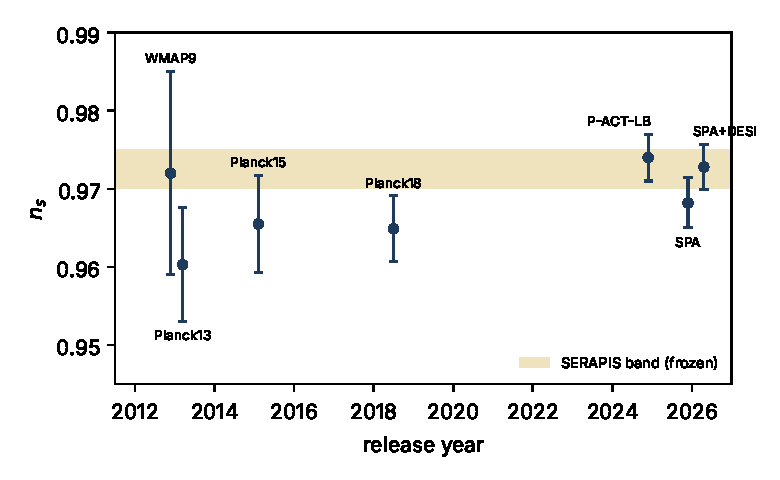
\includegraphics[width=\columnwidth]{figs/fig6_ns_history.pdf}
\caption{Spectral index by data release (WMAP9; Planck 2013, 2015, 2018; ACT DR6 P-ACT-LB; SPT+Planck+ACT without and with DESI BAO) against the frozen SERAPIS band (shaded). The model was fitted after these data; the figure shows consistency, not confirmation.}\label{fig:nshistory}
\end{figure}

\begin{acknowledgments}
\textit{AI assistance.} This work was carried out with substantial help from Claude (Anthropic), a large language model. Claude wrote the analysis code, ran the numerical computations, searched and summarised the literature, and drafted this manuscript and its figures under the author's direction. Results were checked in three ways:
\begin{itemize}
\item every numerical computation was pre-registered in a locked file (group-theory checks excepted; the full list is in MANIFEST.md) with a SHA-256 hash committed before it was run;
\item every correction was logged in a deviations file before any rerun;
\item key outputs were reproduced from a clean state, and every reference was checked against its arXiv record.
\end{itemize}
The author takes full responsibility for the content. Code, pre-registrations and results are archived at Zenodo, doi:10.5281/zenodo.24250733 (Appendix~\ref{app:repro}).
\end{acknowledgments}

\appendix
\section{Reproducibility map}\label{app:repro}
Labels of the form D$nnn$ in the text refer to dated research notes in the public repository (\url{https://github.com/dannyeldridge54/aegis}, branch \texttt{unify-bg}; file \texttt{theory/pending\_docs/D72\_D75\_weak\_spots.md}), where each note records the question, the numbers, the sources and the verdict, with corrections added as separate notes (e.g.\ D585a). Notes that involve a computation have a pre-registration file \texttt{field\_tests/rules/PREREG\_D$nnn$\_*.md}, whose SHA-256 hash was committed before the computation was run, a script in \texttt{theory/modular/}, and an output in \texttt{field\_tests/results/} with the same stem. Table~\ref{tab:repro} lists them. The remaining notes cited (D542, D576, D582, D584, D585, D586, D591, D596, D599, D600, D601, D603, D604, D606, D607, D608, D611, D614, D616, D618, D620, D631) are analytic estimates, reasoning or literature notes that were not pre-registered; D608 includes an unregistered numerical diagnostic, disclosed as such in the note. The scripts that produce the headline numbers and figures can be rerun from \texttt{papers/v3/repro/}.

\begin{table*}[tbp]
\caption{Computations cited in the text up to D639 (later ones are listed in \texttt{MANIFEST.md} and the D-notes): pre-registration (\texttt{PREREG\_}\dots\texttt{.md}) and script (\texttt{.py}; output \texttt{.txt} with the same stem).}\label{tab:repro}
\begin{ruledtabular}
\footnotesize
\begin{tabular}{lll}
Note & Pre-registration & Script \\
\hline
D528 & \texttt{D528\_MODULAR\_PARITY} & \texttt{parity\_d528} \\
D533 & \texttt{D533\_PARITY\_NP} & \texttt{parity\_np\_d533} \\
D551 & \texttt{D551\_VACUUM\_I\_SELECTION} & \texttt{vacuum\_i\_selection\_d551} \\
D564 & \texttt{D564\_SERAPIS\_P} & \texttt{serapis\_p\_d564} \\
D566 & \texttt{D566\_BOUND\_ALPHA} & \texttt{---} \\
D567 & \texttt{D567\_FORWARD\_HOMESAFE} & \texttt{---} \\
D574 & \texttt{D574\_TAU\_I\_DERIVATION} & \texttt{tau\_i\_d574} \\
D575 & \texttt{D575\_TWO\_TERM} & \texttt{two\_term\_d575} \\
D577 & \texttt{D577\_SPECIES\_MASS} & \texttt{species\_mass\_d577} \\
D578 & \texttt{D578\_OSC\_NSTAR} & \texttt{osc\_nstar\_d578} \\
D587 & \texttt{D587\_TWO\_FIELD\_DN} & \texttt{two\_field\_dn\_d587} \\
D588 & \texttt{D588\_EXACT\_NS} & \texttt{exact\_ns\_d588} \\
D589 & \texttt{D589\_N\_COUPLING} & \texttt{n\_coupling\_d589} \\
D592 & \texttt{D592\_ADIABATIC\_Y} & \texttt{adiabatic\_y\_d592} \\
D595 & \texttt{D595\_STIFF\_GROWTH} & \texttt{stiff\_growth\_d595} \\
D597 & \texttt{D597\_S3\_FLAVOUR} & \texttt{s3\_flavour\_d597} \\
D598 & \texttt{D598\_HIGHER\_WEIGHT} & \texttt{higher\_weight\_d598} \\
D602 & \texttt{D602\_EPS\_WINDOW\_LOWTR} & \texttt{eps\_window\_lowtr\_d602} \\
D605 & \texttt{D605\_FORWARD\_TWOTERM} & \texttt{---} \\
D610 & \texttt{D610\_SERAPIS\_RHO\_LOWEPS} & \texttt{serapis\_rho\_d610} \\
D612 & \texttt{D612\_VACUUM\_RHO\_SELECTION} & \texttt{vacuum\_rho\_selection\_d612} \\
D613 & \texttt{D613\_RHO\_NSTAR} & \texttt{rho\_nstar\_d613} \\
D615 & \texttt{D615\_FORWARD\_RHO} & \texttt{---} \\
D632 & \texttt{D632\_RUNNING} & \texttt{running\_d632} \\
D633 & \texttt{D633\_FORWARD\_RUNNING} & \texttt{---} \\
D634 & \texttt{D634\_RHO\_RUNNING} & \texttt{rho\_running\_d634} \\
D635 & \texttt{D635\_JANUS\_ANALYTIC} & \texttt{janus\_analytic\_d635} \\
D637 & \texttt{D637\_KAIROS\_NSTAR} & \texttt{kairos\_nstar\_d637} \\
D639 & \texttt{D639\_SOFT\_MASSES} & \texttt{soft\_masses\_d639} \\
\end{tabular}
\end{ruledtabular}
\end{table*}

\bibliography{refs}
\end{document}
